%% bare_jrnl.tex
%% V1.4a
%% 2014/09/17
%% by Michael Shell
%% see http://www.michaelshell.org/
%% for current contact information.
%%
%% This is a skeleton file demonstrating the use of IEEEtran.cls
%% (requires IEEEtran.cls version 1.8a or later) with an IEEE
%% journal paper.
%%
%% Support sites:
%% http://www.michaelshell.org/tex/ieeetran/
%% http://www.ctan.org/tex-archive/macros/latex/contrib/IEEEtran/
%% and
%% http://www.ieee.org/

%%*************************************************************************
%% Legal Notice:
%% This code is offered as-is without any warranty either expressed or
%% implied; without even the implied warranty of MERCHANTABILITY or
%% FITNESS FOR A PARTICULAR PURPOSE! 
%% User assumes all risk.
%% In no event shall IEEE or any contributor to this code be liable for
%% any damages or losses, including, but not limited to, incidental,
%% consequential, or any other damages, resulting from the use or misuse
%% of any information contained here.
%%
%% All comments are the opinions of their respective authors and are not
%% necessarily endorsed by the IEEE.
%%
%% This work is distributed under the LaTeX Project Public License (LPPL)
%% ( http://www.latex-project.org/ ) version 1.3, and may be freely used,
%% distributed and modified. A copy of the LPPL, version 1.3, is included
%% in the base LaTeX documentation of all distributions of LaTeX released
%% 2003/12/01 or later.
%% Retain all contribution notices and credits.
%% ** Modified files should be clearly indicated as such, including  **
%% ** renaming them and changing author support contact information. **
%%
%% File list of work: IEEEtran.cls, IEEEtran_HOWTO.pdf, bare_adv.tex,
%%                    bare_conf.tex, bare_jrnl.tex, bare_conf_compsoc.tex,
%%                    bare_jrnl_compsoc.tex, bare_jrnl_transmag.tex
%%*************************************************************************

% *** Authors should verify (and, if needed, correct) their LaTeX system  ***
% *** with the testflow diagnostic prior to trusting their LaTeX platform ***
% *** with production work. IEEE's font choices and paper sizes can       ***
% *** trigger bugs that do not appear when using other class files.       ***                          ***
% The testflow support page is at:
% http://www.michaelshell.org/tex/testflow/

\documentclass[journal]{IEEEtran}
%
% If IEEEtran.cls has not been installed into the LaTeX system files,
% manually specify the path to it like:
% \documentclass[journal]{../sty/IEEEtran}

% Some very useful LaTeX packages include:
% (uncomment the ones you want to load)

% *** MISC UTILITY PACKAGES ***
%
%\usepackage{ifpdf}
% Heiko Oberdiek's ifpdf.sty is very useful if you need conditional
% compilation based on whether the output is pdf or dvi.
% usage:
% \ifpdf
%   % pdf code
% \else
%   % dvi code
% \fi
% The latest version of ifpdf.sty can be obtained from:
% http://www.ctan.org/tex-archive/macros/latex/contrib/oberdiek/
% Also, note that IEEEtran.cls V1.7 and later provides a builtin
% \ifCLASSINFOpdf conditional that works the same way.
% When switching from latex to pdflatex and vice-versa, the compiler may
% have to be run twice to clear warning/error messages.






% *** CITATION PACKAGES ***
%
\usepackage{cite}
% cite.sty was written by Donald Arseneau
% V1.6 and later of IEEEtran pre-defines the format of the cite.sty package
% \cite{} output to follow that of IEEE. Loading the cite package will
% result in citation numbers being automatically sorted and properly
% "compressed/ranged". e.g., [1], [9], [2], [7], [5], [6] without using
% cite.sty will become [1], [2], [5]--[7], [9] using cite.sty. cite.sty's
% \cite will automatically add leading space, if needed. Use cite.sty's
% noadjust option (cite.sty V3.8 and later) if you want to turn this off
% such as if a citation ever needs to be enclosed in parenthesis.
% cite.sty is already installed on most LaTeX systems. Be sure and use
% version 5.0 (2009-03-20) and later if using hyperref.sty.
% The latest version can be obtained at:
% http://www.ctan.org/tex-archive/macros/latex/contrib/cite/
% The documentation is contained in the cite.sty file itself.






% *** GRAPHICS RELATED PACKAGES ***
%
\ifCLASSINFOpdf
  \usepackage[pdftex]{graphicx}
  % declare the path(s) where your graphic files are
  % \graphicspath{{../pdf/}{../jpeg/}}
  % and their extensions so you won't have to specify these with
  % every instance of \includegraphics
  % \DeclareGraphicsExtensions{.pdf,.jpeg,.png}
\else
  % or other class option (dvipsone, dvipdf, if not using dvips). graphicx
  % will default to the driver specified in the system graphics.cfg if no
  % driver is specified.
  \usepackage[dvips]{graphicx}
  % declare the path(s) where your graphic files are
  % \graphicspath{{../eps/}}
  % and their extensions so you won't have to specify these with
  % every instance of \includegraphics
  % \DeclareGraphicsExtensions{.eps}
\fi
% graphicx was written by David Carlisle and Sebastian Rahtz. It is
% required if you want graphics, photos, etc. graphicx.sty is already
% installed on most LaTeX systems. The latest version and documentation
% can be obtained at: 
% http://www.ctan.org/tex-archive/macros/latex/required/graphics/
% Another good source of documentation is "Using Imported Graphics in
% LaTeX2e" by Keith Reckdahl which can be found at:
% http://www.ctan.org/tex-archive/info/epslatex/
%
% latex, and pdflatex in dvi mode, support graphics in encapsulated
% postscript (.eps) format. pdflatex in pdf mode supports graphics
% in .pdf, .jpeg, .png and .mps (metapost) formats. Users should ensure
% that all non-photo figures use a vector format (.eps, .pdf, .mps) and
% not a bitmapped formats (.jpeg, .png). IEEE frowns on bitmapped formats
% which can result in "jaggedy"/blurry rendering of lines and letters as
% well as large increases in file sizes.
%
% You can find documentation about the pdfTeX application at:
% http://www.tug.org/applications/pdftex





% *** MATH PACKAGES ***
%
%\usepackage[cmex10]{amsmath}
% A popular package from the American Mathematical Society that provides
% many useful and powerful commands for dealing with mathematics. If using
% it, be sure to load this package with the cmex10 option to ensure that
% only type 1 fonts will utilized at all point sizes. Without this option,
% it is possible that some math symbols, particularly those within
% footnotes, will be rendered in bitmap form which will result in a
% document that can not be IEEE Xplore compliant!
%
% Also, note that the amsmath package sets \interdisplaylinepenalty to 10000
% thus preventing page breaks from occurring within multiline equations. Use:
%\interdisplaylinepenalty=2500
% after loading amsmath to restore such page breaks as IEEEtran.cls normally
% does. amsmath.sty is already installed on most LaTeX systems. The latest
% version and documentation can be obtained at:
% http://www.ctan.org/tex-archive/macros/latex/required/amslatex/math/





% *** SPECIALIZED LIST PACKAGES ***
%
%\usepackage{algorithmic}
% algorithmic.sty was written by Peter Williams and Rogerio Brito.
% This package provides an algorithmic environment fo describing algorithms.
% You can use the algorithmic environment in-text or within a figure
% environment to provide for a floating algorithm. Do NOT use the algorithm
% floating environment provided by algorithm.sty (by the same authors) or
% algorithm2e.sty (by Christophe Fiorio) as IEEE does not use dedicated
% algorithm float types and packages that provide these will not provide
% correct IEEE style captions. The latest version and documentation of
% algorithmic.sty can be obtained at:
% http://www.ctan.org/tex-archive/macros/latex/contrib/algorithms/
% There is also a support site at:
% http://algorithms.berlios.de/index.html
% Also of interest may be the (relatively newer and more customizable)
% algorithmicx.sty package by Szasz Janos:
% http://www.ctan.org/tex-archive/macros/latex/contrib/algorithmicx/




% *** ALIGNMENT PACKAGES ***
%
%\usepackage{array}
% Frank Mittelbach's and David Carlisle's array.sty patches and improves
% the standard LaTeX2e array and tabular environments to provide better
% appearance and additional user controls. As the default LaTeX2e table
% generation code is lacking to the point of almost being broken with
% respect to the quality of the end results, all users are strongly
% advised to use an enhanced (at the very least that provided by array.sty)
% set of table tools. array.sty is already installed on most systems. The
% latest version and documentation can be obtained at:
% http://www.ctan.org/tex-archive/macros/latex/required/tools/


% IEEEtran contains the IEEEeqnarray family of commands that can be used to
% generate multiline equations as well as matrices, tables, etc., of high
% quality.




% *** SUBFIGURE PACKAGES ***
%\ifCLASSOPTIONcompsoc
%  \usepackage[caption=false,font=normalsize,labelfont=sf,textfont=sf]{subfig}
%\else
%  \usepackage[caption=false,font=footnotesize]{subfig}
%\fi
% subfig.sty, written by Steven Douglas Cochran, is the modern replacement
% for subfigure.sty, the latter of which is no longer maintained and is
% incompatible with some LaTeX packages including fixltx2e. However,
% subfig.sty requires and automatically loads Axel Sommerfeldt's caption.sty
% which will override IEEEtran.cls' handling of captions and this will result
% in non-IEEE style figure/table captions. To prevent this problem, be sure
% and invoke subfig.sty's "caption=false" package option (available since
% subfig.sty version 1.3, 2005/06/28) as this is will preserve IEEEtran.cls
% handling of captions.
% Note that the Computer Society format requires a larger sans serif font
% than the serif footnote size font used in traditional IEEE formatting
% and thus the need to invoke different subfig.sty package options depending
% on whether compsoc mode has been enabled.
%
% The latest version and documentation of subfig.sty can be obtained at:
% http://www.ctan.org/tex-archive/macros/latex/contrib/subfig/




% *** FLOAT PACKAGES ***
%
%\usepackage{fixltx2e}
% fixltx2e, the successor to the earlier fix2col.sty, was written by
% Frank Mittelbach and David Carlisle. This package corrects a few problems
% in the LaTeX2e kernel, the most notable of which is that in current
% LaTeX2e releases, the ordering of single and double column floats is not
% guaranteed to be preserved. Thus, an unpatched LaTeX2e can allow a
% single column figure to be placed prior to an earlier double column
% figure. The latest version and documentation can be found at:
% http://www.ctan.org/tex-archive/macros/latex/base/


\usepackage{stfloats}
% stfloats.sty was written by Sigitas Tolusis. This package gives LaTeX2e
% the ability to do double column floats at the bottom of the page as well
% as the top. (e.g., "\begin{figure*}[!b]" is not normally possible in
% LaTeX2e). It also provides a command:
%\fnbelowfloat
% to enable the placement of footnotes below bottom floats (the standard
% LaTeX2e kernel puts them above bottom floats). This is an invasive package
% which rewrites many portions of the LaTeX2e float routines. It may not work
% with other packages that modify the LaTeX2e float routines. The latest
% version and documentation can be obtained at:
% http://www.ctan.org/tex-archive/macros/latex/contrib/sttools/
% Do not use the stfloats baselinefloat ability as IEEE does not allow
% \baselineskip to stretch. Authors submitting work to the IEEE should note
% that IEEE rarely uses double column equations and that authors should try
% to avoid such use. Do not be tempted to use the cuted.sty or midfloat.sty
% packages (also by Sigitas Tolusis) as IEEE does not format its papers in
% such ways.
% Do not attempt to use stfloats with fixltx2e as they are incompatible.
% Instead, use Morten Hogholm'a dblfloatfix which combines the features
% of both fixltx2e and stfloats:
%
% \usepackage{dblfloatfix}
% The latest version can be found at:
% http://www.ctan.org/tex-archive/macros/latex/contrib/dblfloatfix/




%\ifCLASSOPTIONcaptionsoff
%  \usepackage[nomarkers]{endfloat}
% \let\MYoriglatexcaption\caption
% \renewcommand{\caption}[2][\relax]{\MYoriglatexcaption[#2]{#2}}
%\fi
% endfloat.sty was written by James Darrell McCauley, Jeff Goldberg and 
% Axel Sommerfeldt. This package may be useful when used in conjunction with 
% IEEEtran.cls'  captionsoff option. Some IEEE journals/societies require that
% submissions have lists of figures/tables at the end of the paper and that
% figures/tables without any captions are placed on a page by themselves at
% the end of the document. If needed, the draftcls IEEEtran class option or
% \CLASSINPUTbaselinestretch interface can be used to increase the line
% spacing as well. Be sure and use the nomarkers option of endfloat to
% prevent endfloat from "marking" where the figures would have been placed
% in the text. The two hack lines of code above are a slight modification of
% that suggested by in the endfloat docs (section 8.4.1) to ensure that
% the full captions always appear in the list of figures/tables - even if
% the user used the short optional argument of \caption[]{}.
% IEEE papers do not typically make use of \caption[]'s optional argument,
% so this should not be an issue. A similar trick can be used to disable
% captions of packages such as subfig.sty that lack options to turn off
% the subcaptions:
% For subfig.sty:
% \let\MYorigsubfloat\subfloat
% \renewcommand{\subfloat}[2][\relax]{\MYorigsubfloat[]{#2}}
% However, the above trick will not work if both optional arguments of
% the \subfloat command are used. Furthermore, there needs to be a
% description of each subfigure *somewhere* and endfloat does not add
% subfigure captions to its list of figures. Thus, the best approach is to
% avoid the use of subfigure captions (many IEEE journals avoid them anyway)
% and instead reference/explain all the subfigures within the main caption.
% The latest version of endfloat.sty and its documentation can obtained at:
% http://www.ctan.org/tex-archive/macros/latex/contrib/endfloat/
%
% The IEEEtran \ifCLASSOPTIONcaptionsoff conditional can also be used
% later in the document, say, to conditionally put the References on a 
% page by themselves.




% *** PDF, URL AND HYPERLINK PACKAGES ***
%
%\usepackage{url}
% url.sty was written by Donald Arseneau. It provides better support for
% handling and breaking URLs. url.sty is already installed on most LaTeX
% systems. The latest version and documentation can be obtained at:
% http://www.ctan.org/tex-archive/macros/latex/contrib/url/
% Basically, \url{my_url_here}.




% *** Do not adjust lengths that control margins, column widths, etc. ***
% *** Do not use packages that alter fonts (such as pslatex).         ***
% There should be no need to do such things with IEEEtran.cls V1.6 and later.
% (Unless specifically asked to do so by the journal or conference you plan
% to submit to, of course. )


% correct bad hyphenation here
\hyphenation{op-tical net-works semi-conduc-tor}


\begin{document}
%
% paper title
% Titles are generally capitalized except for words such as a, an, and, as,
% at, but, by, for, in, nor, of, on, or, the, to and up, which are usually
% not capitalized unless they are the first or last word of the title.
% Linebreaks \\ can be used within to get better formatting as desired.
% Do not put math or special symbols in the title.
\title{A Gait Analysis Software as a Service}
%
%
% author names and IEEE memberships
% note positions of commas and nonbreaking spaces ( ~ ) LaTeX will not break
% a structure at a ~ so this keeps an author's name from being broken across
% two lines.
% use \thanks{} to gain access to the first footnote area
% a separate \thanks must be used for each paragraph as LaTeX2e's \thanks
% was not built to handle multiple paragraphs
%

\author{
	Roberto~Aguiar~Lima,
	Vera~Regina~Fernandes~Da~Silva~Maraes,
	Jairo Simao Santana Melo,
	Vladimir Franca Nogueira,
        and~Lourdes~Mattos~Brasil,~\IEEEmembership{Member,~IEEE.}
	\thanks{R. A. Lima, V. R. S. Maraes and L. M. Brasil are with Biomedical Engineering Post Graduate Program, University of Brasilia at Gama, DF.}
	\thanks{J. S. S. Melo is with Federal District Court of Law, Brasilia, DF.}
	\thanks{V. F. Nogueira is with Universidade of Brasilia at Gama, DF.}
	\thanks{Manuscript received October ??, ????; revised December ?, ????.}
}


% note the % following the last \IEEEmembership and also \thanks - 
% these prevent an unwanted space from occurring between the last author name
% and the end of the author line. i.e., if you had this:
% 
% \author{....lastname \thanks{...} \thanks{...} }
%                     ^------------^------------^----Do not want these spaces!
%
% a space would be appended to the last name and could cause every name on that
% line to be shifted left slightly. This is one of those "LaTeX things". For
% instance, "\textbf{A} \textbf{B}" will typeset as "A B" not "AB". To get
% "AB" then you have to do: "\textbf{A}\textbf{B}"
% \thanks is no different in this regard, so shield the last } of each \thanks
% that ends a line with a % and do not let a space in before the next \thanks.
% Spaces after \IEEEmembership other than the last one are OK (and needed) as
% you are supposed to have spaces between the names. For what it is worth,
% this is a minor point as most people would not even notice if the said evil
% space somehow managed to creep in.



% The paper headers
\markboth{IEEE TRANSACTIONS ON NEURAL SYSTEMS AND REHABILITATION ENGINEERING,~Vol.~??, No.~?, ?????????~201?}%
{Shell \MakeLowercase{\textit{et al.}}: Bare Demo of IEEEtran.cls for Journals}
% The only time the second header will appear is for the odd numbered pages
% after the title page when using the twoside option.
% 
% *** Note that you probably will NOT want to include the author's ***
% *** name in the headers of peer review papers.                   ***
% You can use \ifCLASSOPTIONpeerreview for conditional compilation here if
% you desire.




% If you want to put a publisher's ID mark on the page you can do it like
% this:
%\IEEEpubid{0000--0000/00\$00.00~\copyright~2014 IEEE}
% Remember, if you use this you must call \IEEEpubidadjcol in the second
% column for its text to clear the IEEEpubid mark.



% use for special paper notices
%\IEEEspecialpapernotice{(Invited Paper)}




% make the title area
\maketitle

% As a general rule, do not put math, special symbols or citations
% in the abstract or keywords.
\begin{abstract}
	This paper presents the implementation of a human gait analysis Software as a Service (SaaS).
	This approach has as advantage, the software availability at the web.
	After the software is implanted at a webserver, users may access it from a recent
	web browser with HTML5 support.
	The goal of software is to minimize code development efforts of researchers from gait analysis, 
	as well as to be useful tool for health professionals interested in the human gait analysis.
	The software allows import positional data from a third party motion captures system,
	that uses surface markers and video cameras, to plot markers spatial progression, 
	angles, angular velocities and angular accelerations. Furthermore, it is possible
	to see and to interact with a 3D animation from markers. 
	The software source code is available as free software,
	often receive new features and a new community is being created to maintain it.
\end{abstract}

% Note that keywords are not normally used for peerreview papers.
\begin{IEEEkeywords}
Gait analysis, software as a service, SaaS.
\end{IEEEkeywords}

% For peer review papers, you can put extra information on the cover
% page as needed:
% \ifCLASSOPTIONpeerreview
% \begin{center} \bfseries EDICS Category: 3-BBND \end{center}
% \fi
%
% For peerreview papers, this IEEEtran command inserts a page break and
% creates the second title. It will be ignored for other modes.
\IEEEpeerreviewmaketitle



\section{Introduction}
% The very first letter is a 2 line initial drop letter followed
% by the rest of the first word in caps.
% 
% form to use if the first word consists of a single letter:
% \IEEEPARstart{A}{demo} file is ....
% 
% form to use if you need the single drop letter followed by
% normal text (unknown if ever used by IEEE):
% \IEEEPARstart{A}{}demo file is ....
% 
% Some journals put the first two words in caps:
% \IEEEPARstart{T}{his demo} file is ....
% 
% Here we have the typical use of a "T" for an initial drop letter
% and "HIS" in caps to complete the first word.
\IEEEPARstart{W}{ith} the advent of software web, is possible to create services
that are placed at webservers and access it  from anywhere.
Furthermore, modern web browsers have become a truly platform, which allows
create rich interfaces that include graphical presentation and 3D animations
without the need of plugins installations.
% You must have at least 2 lines in the paragraph with the drop letter
% (should never be an issue)
These two technologies, web browsers and webservers, may be used to build
what is known as Software as a Service (SaaS). The SaaS advantages for 
customers and software developers are \cite{Fox2012}: customers do not need
to install the application; data associated with the service should be kept centralized,
so it is protected; data may be collectively accessed by a group of users;
big datasets and data that is frequently updated, are kept centralized 
and remote access to them are offered; only a single copy of the server software
runs in a controlled hardware and operating system environment, which avoids
compatibility problems, in addition, new versions of the software can be 
tested with a small fraction of the real customers without disturbing most
customers.

Although there was advances on the gait analysis by the middle of century XX, 
clinic gait analysis became broadly available only
with the modern computer advent \cite{Baker2007}.
Actually, there are a lot of software packages for this purpose \cite{Moraes2003}.
But until now there are no software provider committed to deliver a 
gait analysis SaaS. in other words, health professionals or gait analysis researchers
who need to use software, must install it at specific hardware and
operating system. Furthermore, they have to be responsible by data backup and if there are
new software versions, it must be installed again. Whether they
need to share data, then must copy and send it to the destiny. In addition, others
security concerns must be addressed as well.
These problems may be minimized or even eliminated with a SaaS.

In order to implement a software is essential to accomplish the requirements elicitation 
and a certain domain of the field should be understood, in this case gait analysis. 
Nowadays, the theme is quite documented
\cite{Perry2010, Whittle2012, Ferreira2009, Vieira2015, 
Duhamel2004, Ghoussayni2004, Moreno2009, Beynon2010}. 
Moreover, there are experienced health professionals in the development
with knowledge on gait analysis. 
Then, this paper presents the
first implementation version of a gait analysis SaaS \cite{Lima2015}.
This software version may import data from a third party motion capture system, in this
case data collected from video cameras using surface markers. Also the software
may name markers, define angles, and plot 
markers progression at space, angles, angular velocities and angular accelerations.
So, the software presents a 3D animation from imported data and allows user 
interact with it.


% needed in second column of first page if using \IEEEpubid
%\IEEEpubidadjcol

\section{Materials and Methods}

Two researches environments were used to undertake the project. 
One was the Human Performance Lab (\emph{Laboratório de Performance Humana} - LPH) in
University of Brasilia (\emph{Universidade de Brasilia} - UnB) at Ceilandia, 
and the other was the Health Informatics Lab (\emph{Laboratorio de Informatica em Saude} - LIS)
in UnB at Gama. 
Data acquisition was made in LPH and software development tasks at LIS.

The next subsections presents the process for data acquisition,
the development process and the general
view of the software architecture.

\subsection{Data Acquisition}

The data are acquired by sixteen Qualisys Oqus cameras that use
the Qualisys Track Manager Software (QTM). 
The data are relative to surface markers along a patient's body.

For this paper a healthy patient, male, with age between 20 and 30 years old
was selected.
Fig. \ref{data_acq_proc} summarizes the data acquisition process.
First,  the  markers positions are defined by the gait analysis specialist. 
For this paper, only the left trochanter, left knee and left tibia
positions were considered. 
So the surface markers must be set at defined positions on patient's body.
The next step is acquire data from the cameras and QTM software. In this
step, the patient performs a comfortable gait cycle in front of the cameras.
Then, five gait samples were acquired.
The last step is convert the acquired data to MATLAB format that use the QTM
software. Furthermore, it is important due to the standard chosen for 
the gait analysis software.

The process for data acquisition was approved by Ethics Committee from Faculty of Health 
\emph{Faculdade de Saude} / UnB  
process number N11911/12.

\begin{figure}[!t]
	\centering
	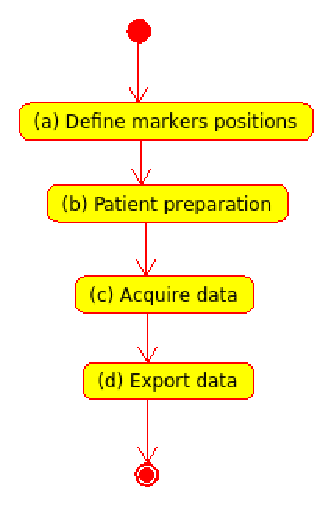
\includegraphics[width=1.5in]{./data_acq_proc.eps}
	\caption{Data acquisition process.
		(a) Positions of markers to be fixed in patient body are defined;
		(b) Markers are fixed at defined positions;
		(c) Patient executes some comfortable gait cycles in front of cameras.
		QTM software is used;
		(d) Data acquired are converted to MATLAB format using QTM software.
	}
	\label{data_acq_proc}
\end{figure}


\subsection{Development Process}

A scrum \cite{Schwaber2001, Schwaber2004, Rubin2012} inspired process for development was implanted.
The scrum is a agile method \cite{Beck2001} that has as mainly characteristics
to be iterative, incremental and change friendly.
These characteristics are essentials to deal with software requirements volatility
and, hence, with software changes.

The process flow is presented in Fig. \ref{dev_proc}.
These process consist of iterations called sprints.
The sprints have a 2 weeks average duration.
Therefore, a product backlog is created and managed by the product owner.
Also the product backlog is open to receive additions from any
project stakeholders, at any time, but only the product owner may prioritize it,
that are based in expected values for final users.
Each item at the product backlog is a user story \cite{cohn2004}.

Before a new iteration begins, there are a two phases meeting between the development team members. 
In the first phase, the last increment is presented and 
impediments occurred in the last iteration are revealed.
In the second phase, the development team selects items from the product backlog.
These items will be implemented in the sprint and are called the sprint backlog.
Finally , is delivered an increment that consist in a piece of working software.

\begin{figure}[!t]
	\centering
	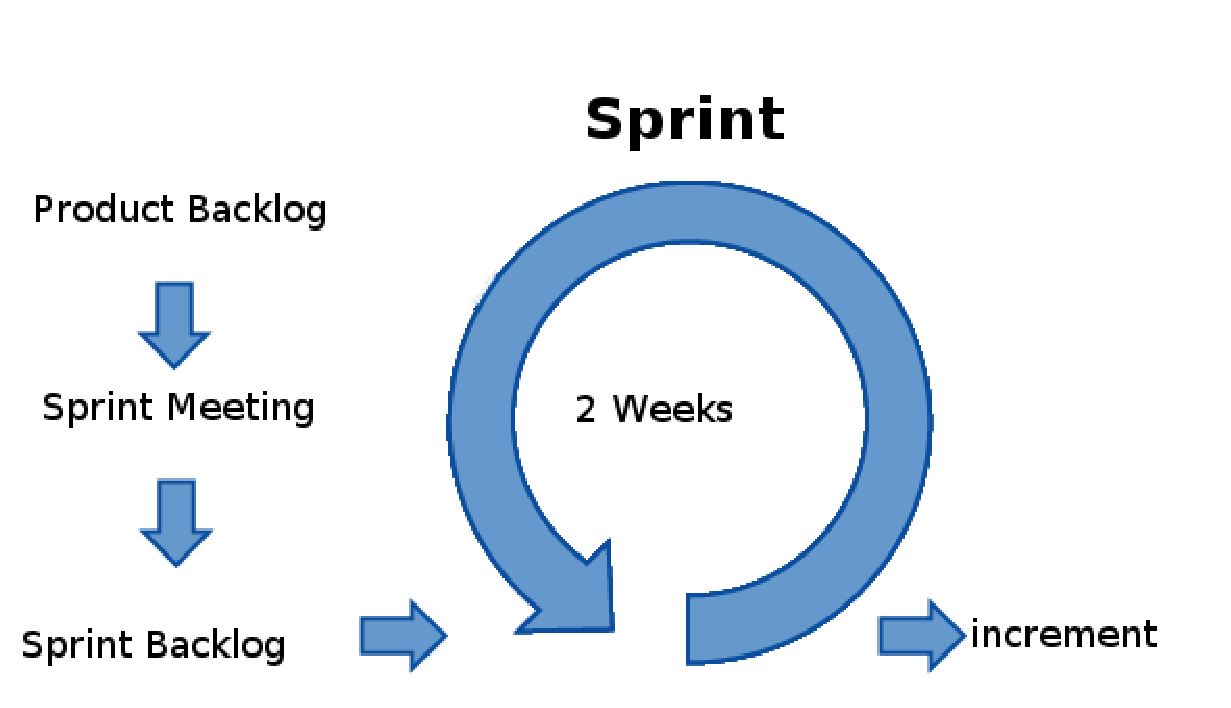
\includegraphics[width=0.48\textwidth]{./dev_proc.eps}
	\caption{Development process overview.
		Every two weeks a new increment, working software, is delivered.
		Adapted from \cite{Schwaber2004}.
	}
	\label{dev_proc}
\end{figure}

\subsection{Software Architecture General View}
The Fig. \ref{app_layers} shows the software architecture layered high level view.
The web applications layer is responsible by application user interactions (Section \ref{web_application_layer}).
The layer REST web API is responsible by business logic, (Section \ref{rest_web_api_layer}).
The document base layer is responsible by data application persistence (Section \ref{document_base_layer}).
\begin{figure}[!t]
	\centering
	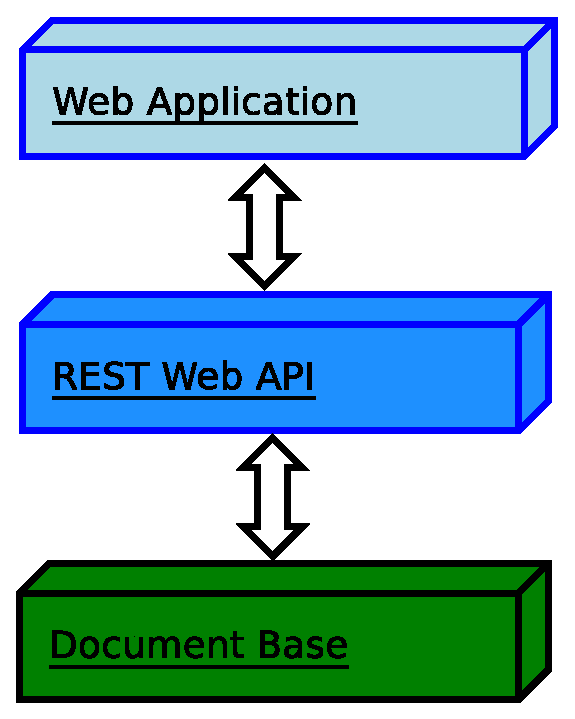
\includegraphics[width=2in]{./app_layers.eps}
	\caption{The high level view of the software architecture layered.
	}
	\label{app_layers}
\end{figure}

\subsubsection{Web Application Layer}
\label{web_application_layer}

This layer was designed to run in web browsers with HTML5 support.
It was developed with Javascript, CSS and HTML languages. 
Moreover, the web development framework AngularJS was adopted \cite{Branas2014,Freeman2014}. 
A great AngularJS adoption advantage is the directive creation possibility. 
Directives are developed components which may be embedded in a HTML template.
Also, it was chosen to use the Angular-Material directive library. 
This library is based in the Material Design specification from Google, which
describes about graphical design patterns and user interaction, it is based in the material metaphor
\cite{Google2015a}. The Angular-Material use, so it is possible to build a user experience that are acceptable by health professionals.

The ThreeJS library was chosen to run graphical 3D animations \cite{Dirksen2015}.
This is a high level library for computer graphics, 
which takes advantage from WebGL implementation in modern web browsers.
The WebGL specification \cite{Matsuda2013} uses the computer Graphical Processor Unit (GPU) natively, 
that allows to build applications which needs good performance to generate animations and graphics.

\begin{figure*}[tb]
	\centering
	{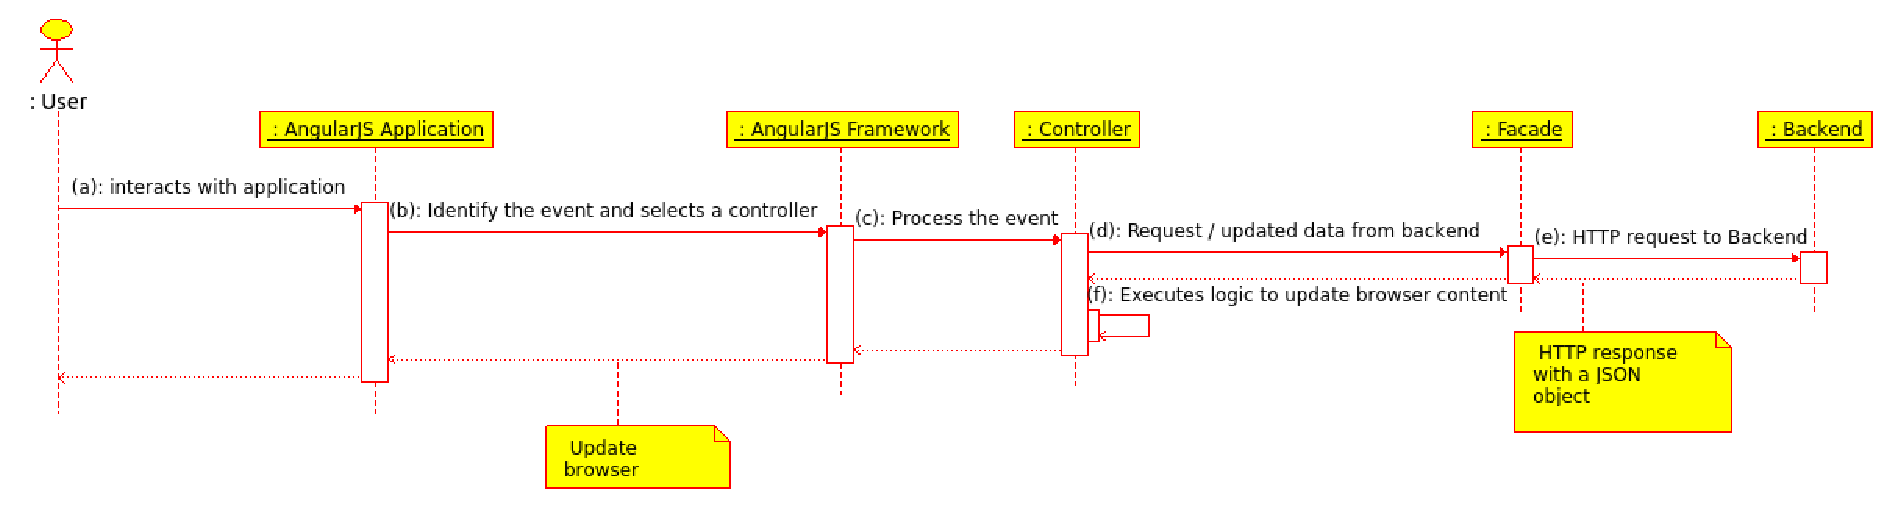
\includegraphics[width=0.95\textwidth]{./web_components.eps}}
	\caption{Main web application layer components interactions.
		All these components, except the component backend, run inside the web browses.
		The component backend correspond to the infrastructure and components of REST web API layer.
		(a) A user interacts with the application, for example, a click button on screen;
		(b) The AngularJS framework detects the event, selects a controller component and
		dispatch the event for it;
		(c) The selected controller process the event;
		(d) If it is necessary to execute some action, as request more data, the controller 
		requests to a facade component to requests the backend;
		(e) The selected facade component prepares and send a HTTP request to the backend,
		which returns a JSON object;
		(f) The controller updates the model, variables used by the framework to show data at screen,
		and signals to the AngularJS framework to update the screen.
	}
	\label{web_components}
\end{figure*}

\begin{figure*}[tb]
	\centering
	{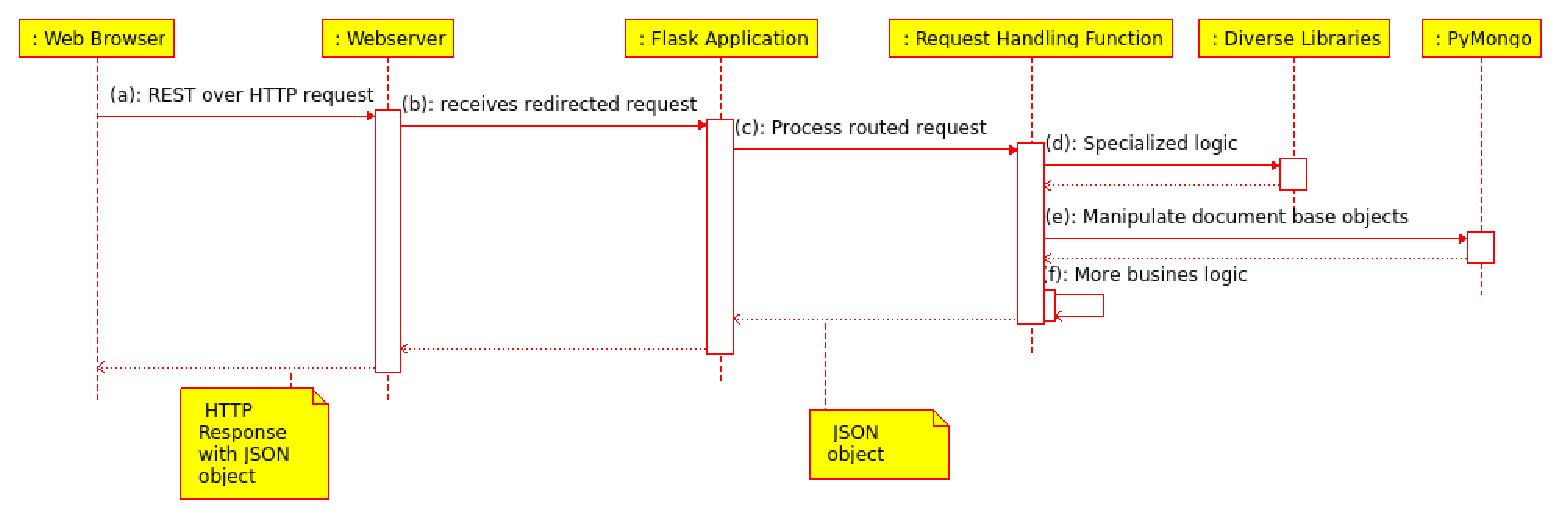
\includegraphics[width=0.95\textwidth]{./rest_web_api_components.eps}}
	\caption{Main REST web API layer components interactions.
		(a) From the user web browser, a HTTP request is sent to the  webserver that runs the web API;
		(b) The webserver redirects the request to the Flask Application.  
		(c) The flask application routes the request to the appropriate handling function;
		(d) If necessary the handling function access specialized libraries, like NumPy,
		Matplotlib or a library for business logic, for example,
		to calculate kinematics from gait data;
		(e) If data manipulation from document base layer is needed, calls to PyMongo can be made; 
		(f) The function handling may implement business logic too, but it is only advise for simple
		things. The return data is encapsulated like a JSON object end sent to the webserver to
		complete the original request from the web browser.
	}
	\label{rest_web_api_components}
\end{figure*}

Fig. \ref{web_components} shows the interaction between  main components in web application layer.
It can be observed that this is only a logic representation.
When a user interacts with the application in the web browser, it produces events detected by the 
AngularJS framework. The interaction may be a button click event, a mouse over event, a drag event or
other. So, the framework selects a controller component to process the event.
Controllers are components developed to the application, these are responsible to coordinate
data access to the model and to update the view. 

AngularJS applications use a famous design pattern called Model-View-Controller \cite{Fowler2002}. 
In practice, this means that controllers update the application state, so the AngularJS framework
should update the screen to users.
If new data or business logic execution are relevant, the controller request to a facade component
that communicate with the backend. 
Facade is a design pattern which hides complex logic required to perform some action \cite{Fowler2002}. 
In this case is the communication over HTTP protocol to the backend.
After the backend receives the request, it process and sends a HTTP response with a JSON object inside.
JavaScript Object Notation (JSON) are a specification to represent and exchange data.

\subsubsection{REST Web API Layer}
\label{rest_web_api_layer}

This layer is responsible to execute business logic, for example,
calculate angles, extract data   from QTM software, among others.
The layer was implemented using the architectural style Representational State Transfer (REST) 
\cite{Grinberg2014}.
The main advantage of this technology is the high decoupling with the web application layer.
This decoupling promotes concepts separation between these layers, improving development process
and application maintainability.
To implement the REST style, was chosen the framework Flask \cite{Maia2015}.
Flask is implemented in Python language, it is known by minimalist philosophy 
that allows to create a simple project, which evolves into more complex models, according with
requisites at moment.

Fig. \ref{rest_web_api_components} shows the interaction between  main components in REST web API layer.
This representation is only a logic view.
After a user interacts with web application run at web browser and an action from the REST web API is
needed, a HTTP request is sent to the webserver. This is a REST style request.
The webserver receives the request and verify it. If, this request to the web API is  yes, the
request is dispatched to the web API implementation, that is written by the framework Flask.
The framework Flask identifies the request and selects the appropriate handling function. 
This function is written in Python language. 
The request handling function may access many libraries, like NumPy for number crunching,
Matplotlib for generate scientific graphics that are be sent to the user. 
Business logic application specific libraries may also be used, like libraries to calculate
cinematic information;
The PyMongo is an important library that may be used by the handling function as well.
This component will access the document base manager MongoDB (Section \ref{document_base_layer}),
so is possible manipulate and persist the application data.
The request handling also implements business logic, but is advised to implement complex logic in a specific
library.
When entire processing is done, a response is generated as a JSON object and sent back to 
the web application that runs at the user browser.
\subsubsection{Document Base Layer}
\label{document_base_layer}

The data persistence and basic manipulation is done by the document base layer.
This layer comprises a server running the document base manager MongoDB 
\cite{Plugge2014}, \cite{Plugge2014}.
This technology was chosen instead of a relational database management system, 
because the multidimensional data scope of the application is easily  modeled with
a document base. Also MongoDB is more easily scalable than a relational database management system.
MongoDB does not use tables like relational databases, it uses the collection concept.
A collection is a set of objects. Objects of a collection may have different structures
or types, although this is a bad practice. A MongoDB database can have multiple collections.
Objects are expressed using de BSON notation, which are very similar to JSON.

The Fig. \ref{mongo_oga} shows the application data base.
It have two data collections: patients and positionals\_data.
The patients collections have basic data from the patient.
The positionals\_data collection has spatial and markers 
data imported from a QTM/MATLAB file.
\begin{figure}[!t]
	\centering
	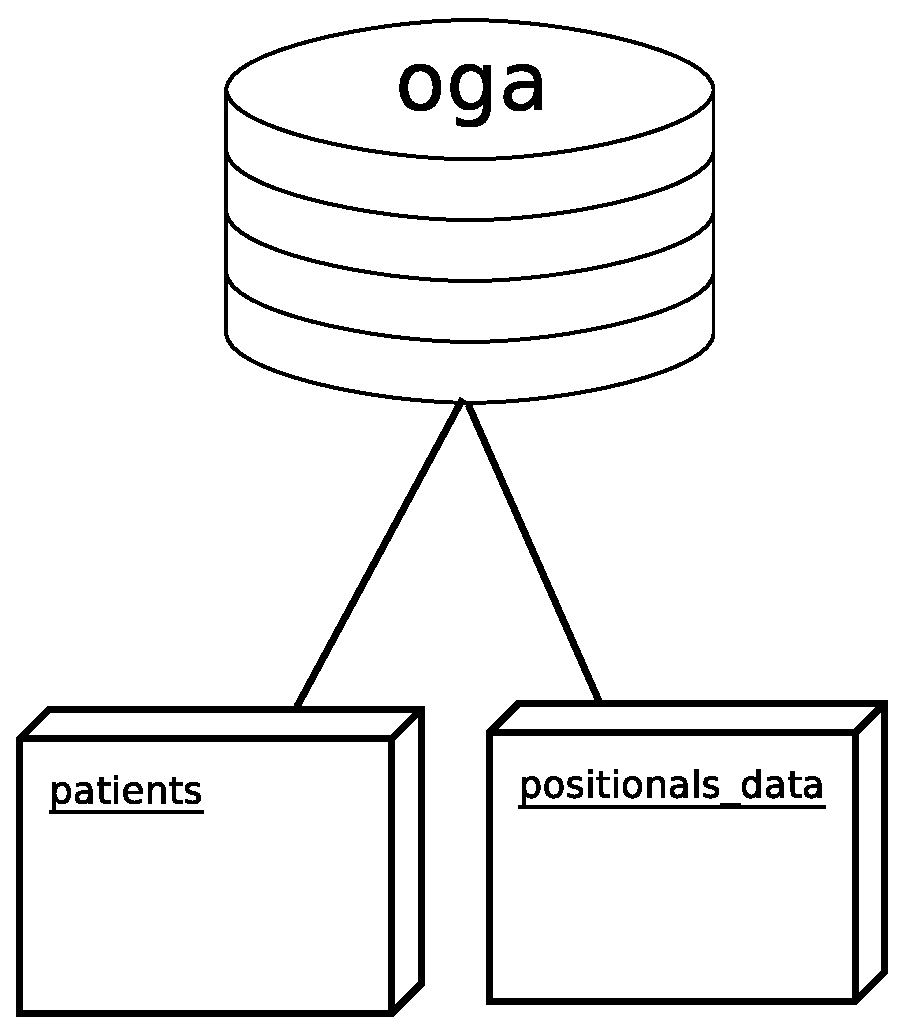
\includegraphics[width=1.5in]{./mongo_oga.eps}
	\caption{Application document base. The data base name is "oga". 
	This database has two collections: patients and positionals\_data. 
	}
	\label{mongo_oga}
\end{figure}


\section{Results}

The developed software allows to register patients.
After the patient is registered, the user may include gait samples to this patient.
This sample is imported to the software from a MATLAB file generated by the QTM software.
After the file is imported the screen described in Fig. \ref{qtm_data} is shown.
From this screen is possible to run a 3D animation including the markers acquired (Fig. \ref{animation}).
There is possible accelerate or slowdown the animation, to apply zoom in or zoom out, to controller pan
and to see a specific frame in the animation.
It is am important feature to see a frame because may be used to visualize the initial contact
and terminal swing frames. 
So, it is possible to update these fields in the screen shown at Fig. \ref{qtm_data}(c).
These data fields must be correctly filled otherwise the graphics will be incorrect.


The software has an option to name markers. After a marker is named, a graphic showing the 
marker's spatial progression will be plotted (Fig. \ref{spatial_progression}). 
Another important feature is the angle registering tool (Fig.~\ref{angles_tool}). 
After an angle is registered (Fig.~\ref{angles}), angular velocities (Fig.~\ref{av}) 
and angular accelerations (Fig.~\ref{aa}) will be plotted.

Another advantage of AngularJS and Material-Angular is the seamless adaptation of their components to small screens. This characteristic turns possible with little effort to adapt the application to mobile phones.
The Fig. \ref{iphone} shows the application running in a mobile phone.

\section{Discussion}

A software for gait analysis fully available at web is a innovation in the field.
The bigger advantage is the easy access to the software,
because after the application is implanted in an internet webserver, 
a user with a recent HTML5 browser can use the application, independent from
the location.

Another theme that raises from this project is the creation of a centralized 
base, with data collected around world. Such endeavor would be priceless
to gait analysis researchers. This would require a more profound care with 
information security.

The software is available as free software. The intention is to attract
developers and health professionals to contribute and to use the software.

As future works, new data acquisition methods should be implemented, as plate force, electromyography (EMG)
and inertial measurement unit (IMU). 
The inclusion of automatic detection events at gait cycle could be a plus, for example,
detect the initial contact and terminal swing.
Furthermore, a simulation module is being developed. 
It will support machine learning methods to regression and classification.


\section{Conclusion}
This paper presented a gait analysis SaaS. It source code is available as free software 
under the MIT license \cite{MIT2015} at the web address <http://github.com/rob-nn/open\_gait\_analytics>.

The software offers data importation from the third party software QTM from Qualisys.
These data are about surface markers fixed in a patient body.
The software allows name markers, plot a spatial progression from it.
Also is possible to register angles and show graphics with angular velocities and angular accelerations.
The markers may be viewed by 3D animation.
All graphics are displayed according to the gait cycle phases.

The software will continue receive more features, and gradually will be available for more users.
It is possible to other people implant or use the software as they wish.

% use section* for acknowledgment
\section*{Acknowledgment}

The first author would like to thank the financial support granted by CAPES.
The authors would like to thank LIS UnB at Gama and LPH UnB at Ceilandia,
by use of its resources.

\begin{figure*}[tb]
	\centering
	{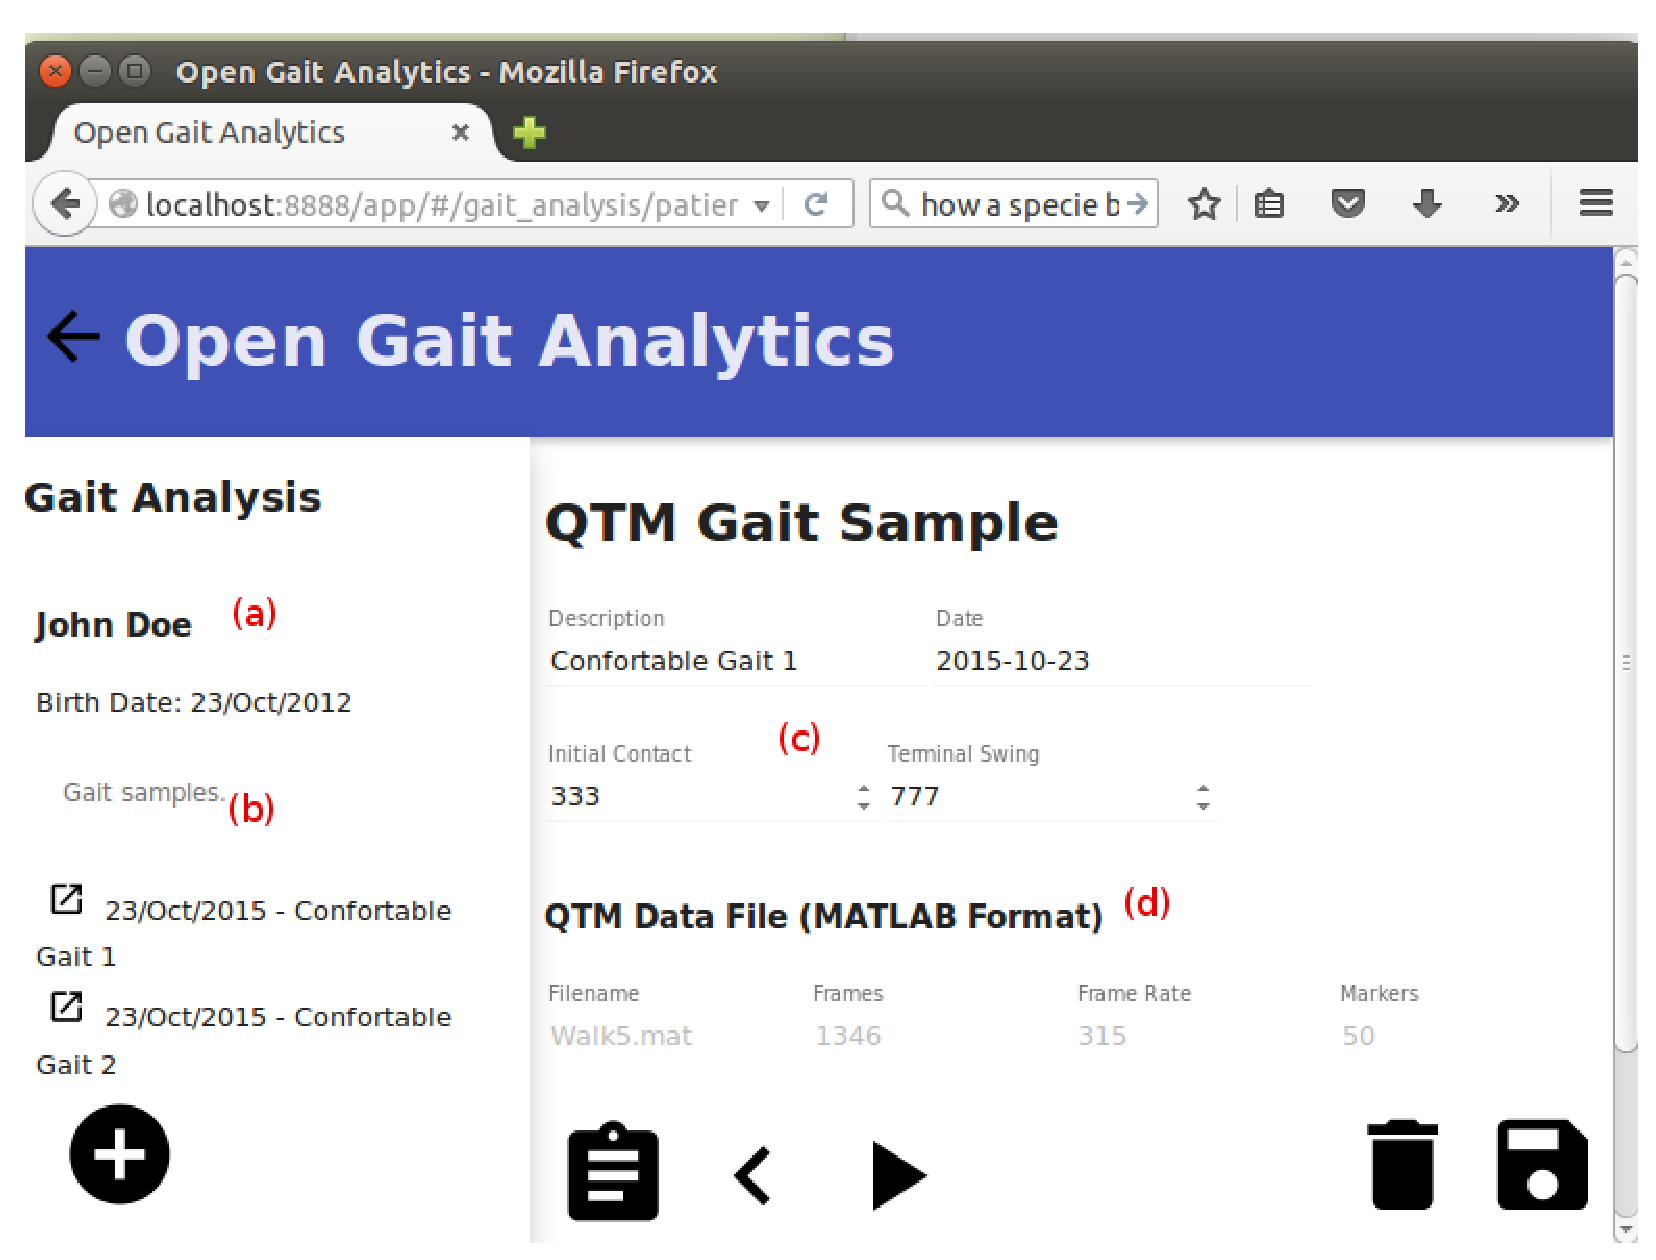
\includegraphics[width=0.6\textwidth]{./qtm_data.eps}}
	\caption{Gait analysis screen. 
		(a) Patient name;
		(b) Gait samples acquired from the patient and imported to the software;
		(c) Initial contact and terminal swing frames must be informed by the user,
		which may use the animation feature to know the correct frames;
		(d) QTM imported file summary.
	}
	\label{qtm_data}
\end{figure*}


\begin{figure*}[tb]
  \centering
  \begin{minipage}[b]{0.32\textwidth}
    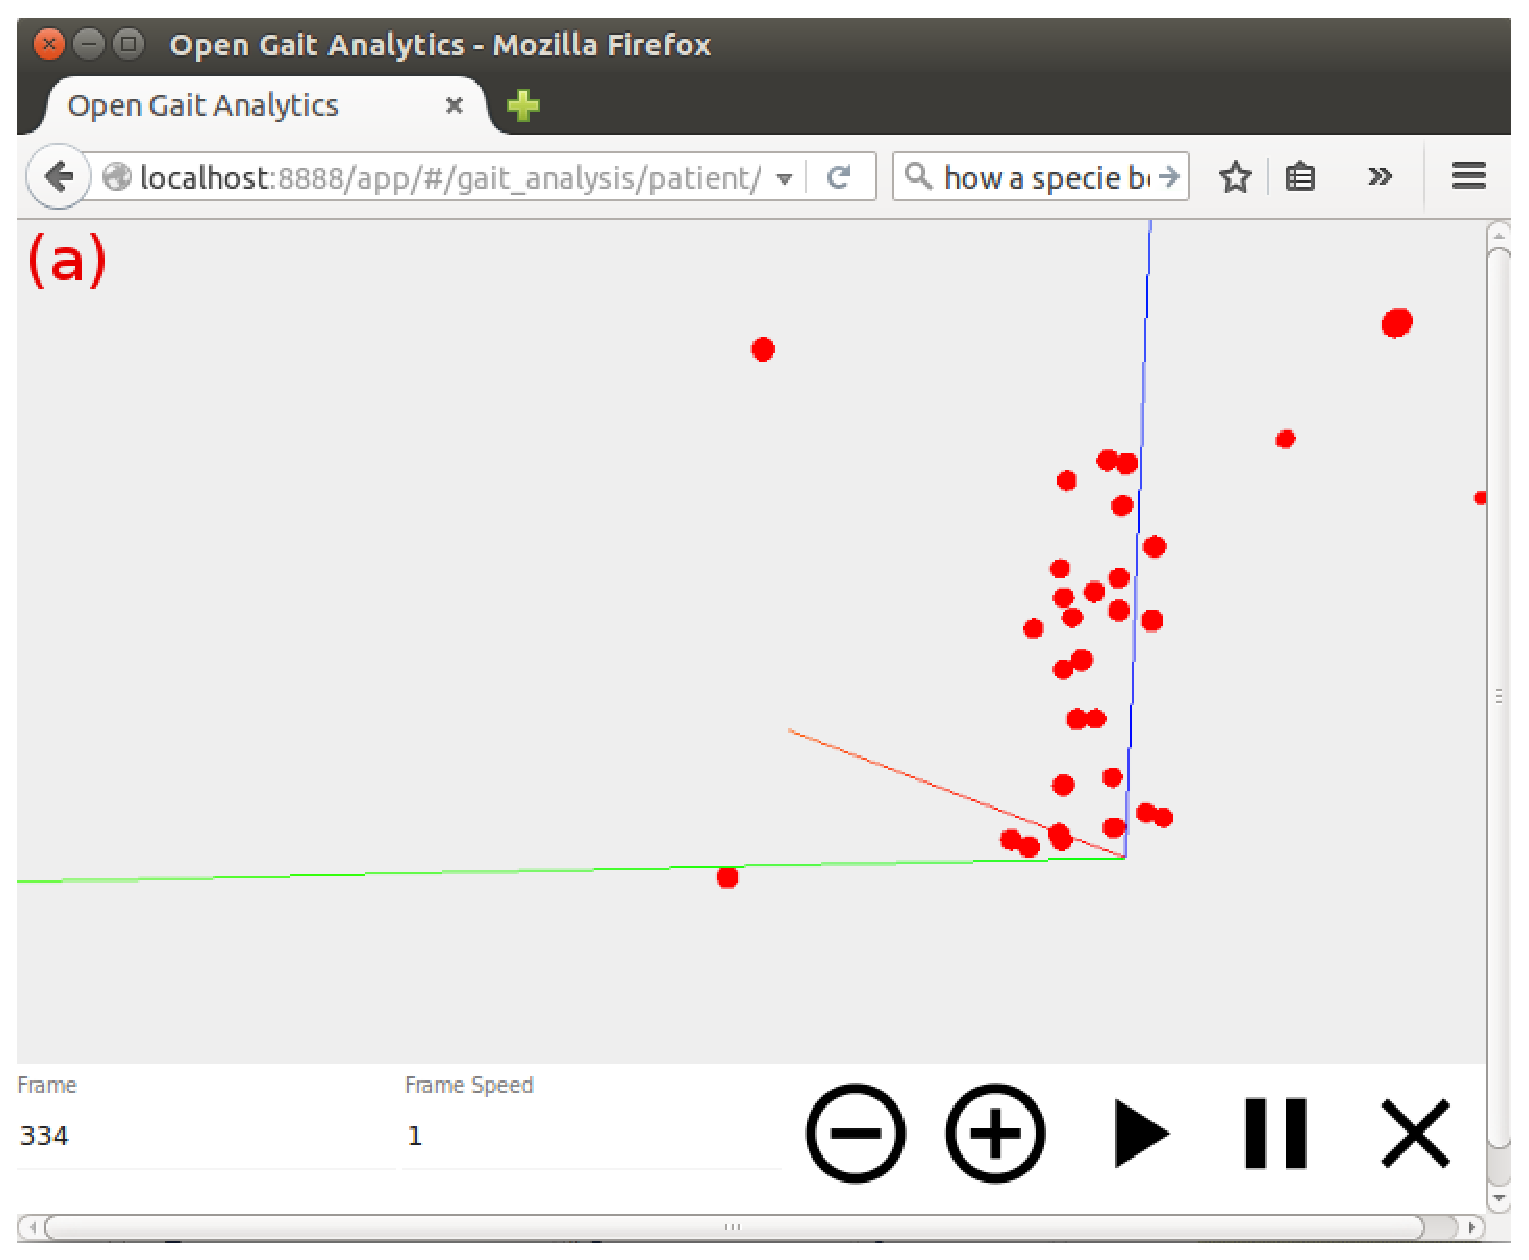
\includegraphics[width=\textwidth]{./animation1.eps}
  \end{minipage}
  \hfill
  \begin{minipage}[b]{0.32\textwidth}
    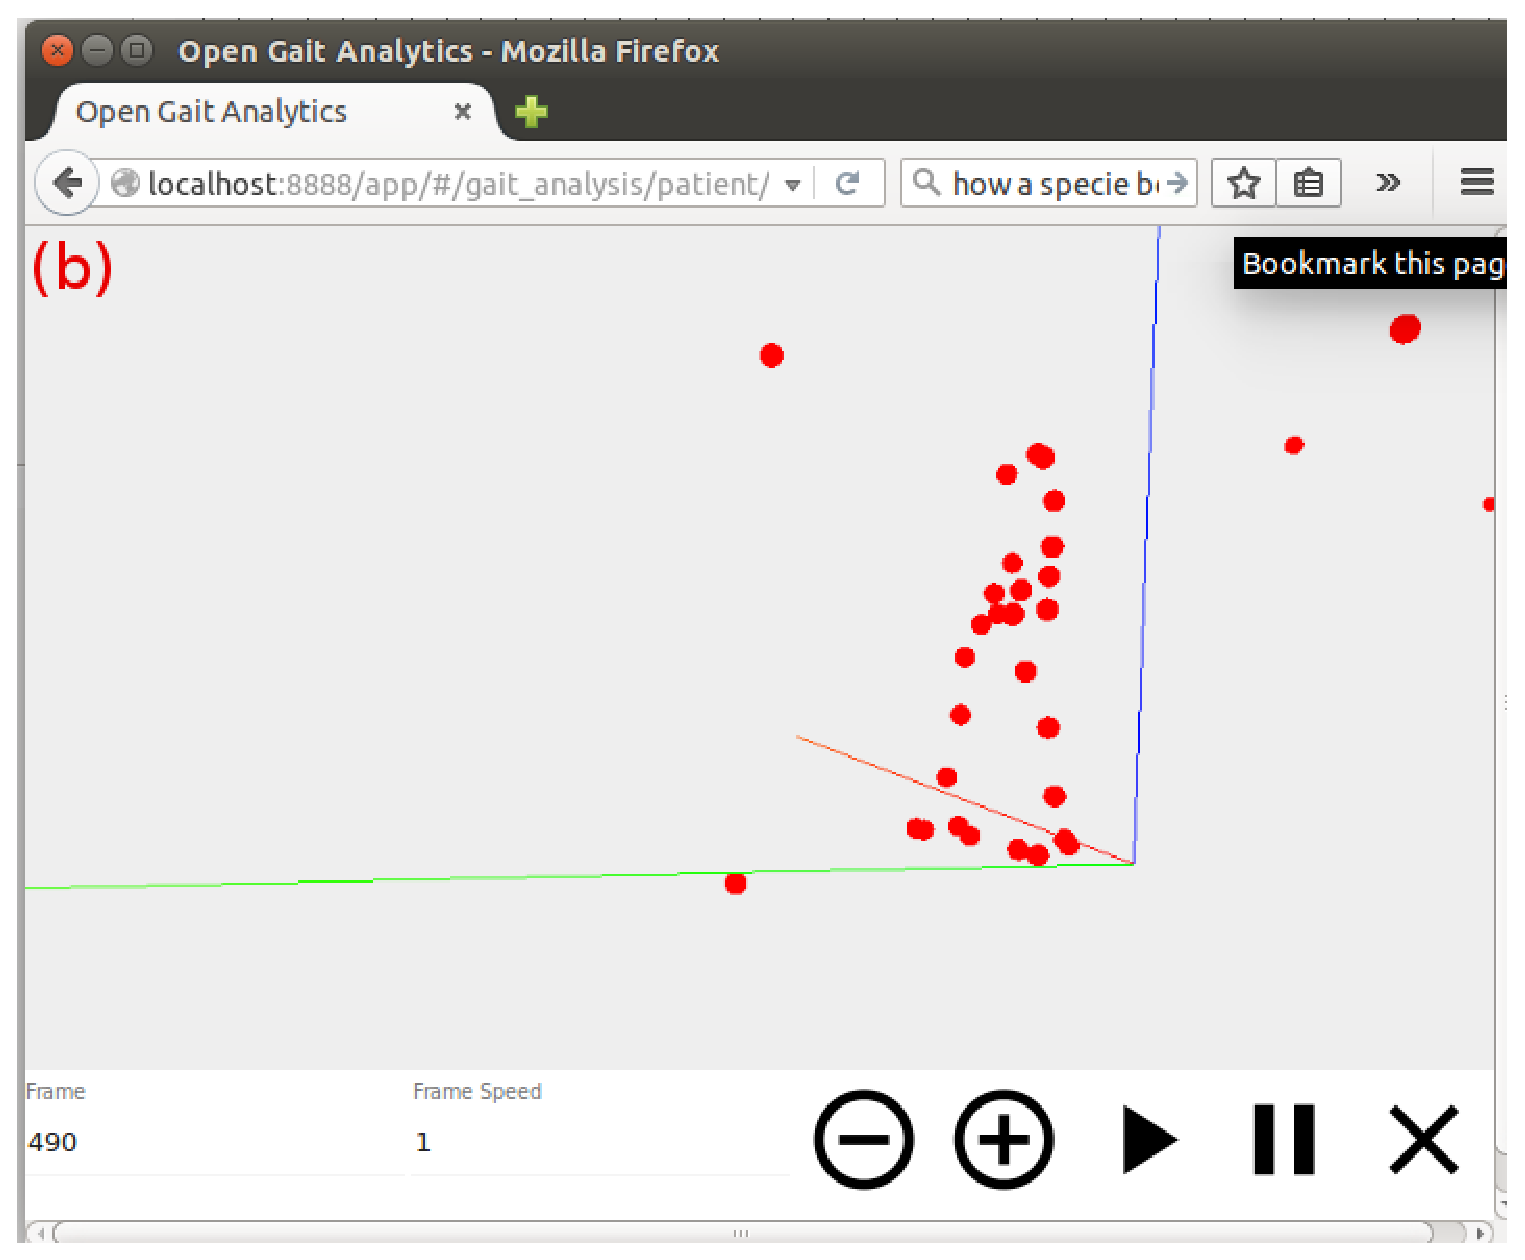
\includegraphics[width=\textwidth]{./animation2.eps}
  \end{minipage}
  \hfill
  \begin{minipage}[b]{0.32\textwidth}
    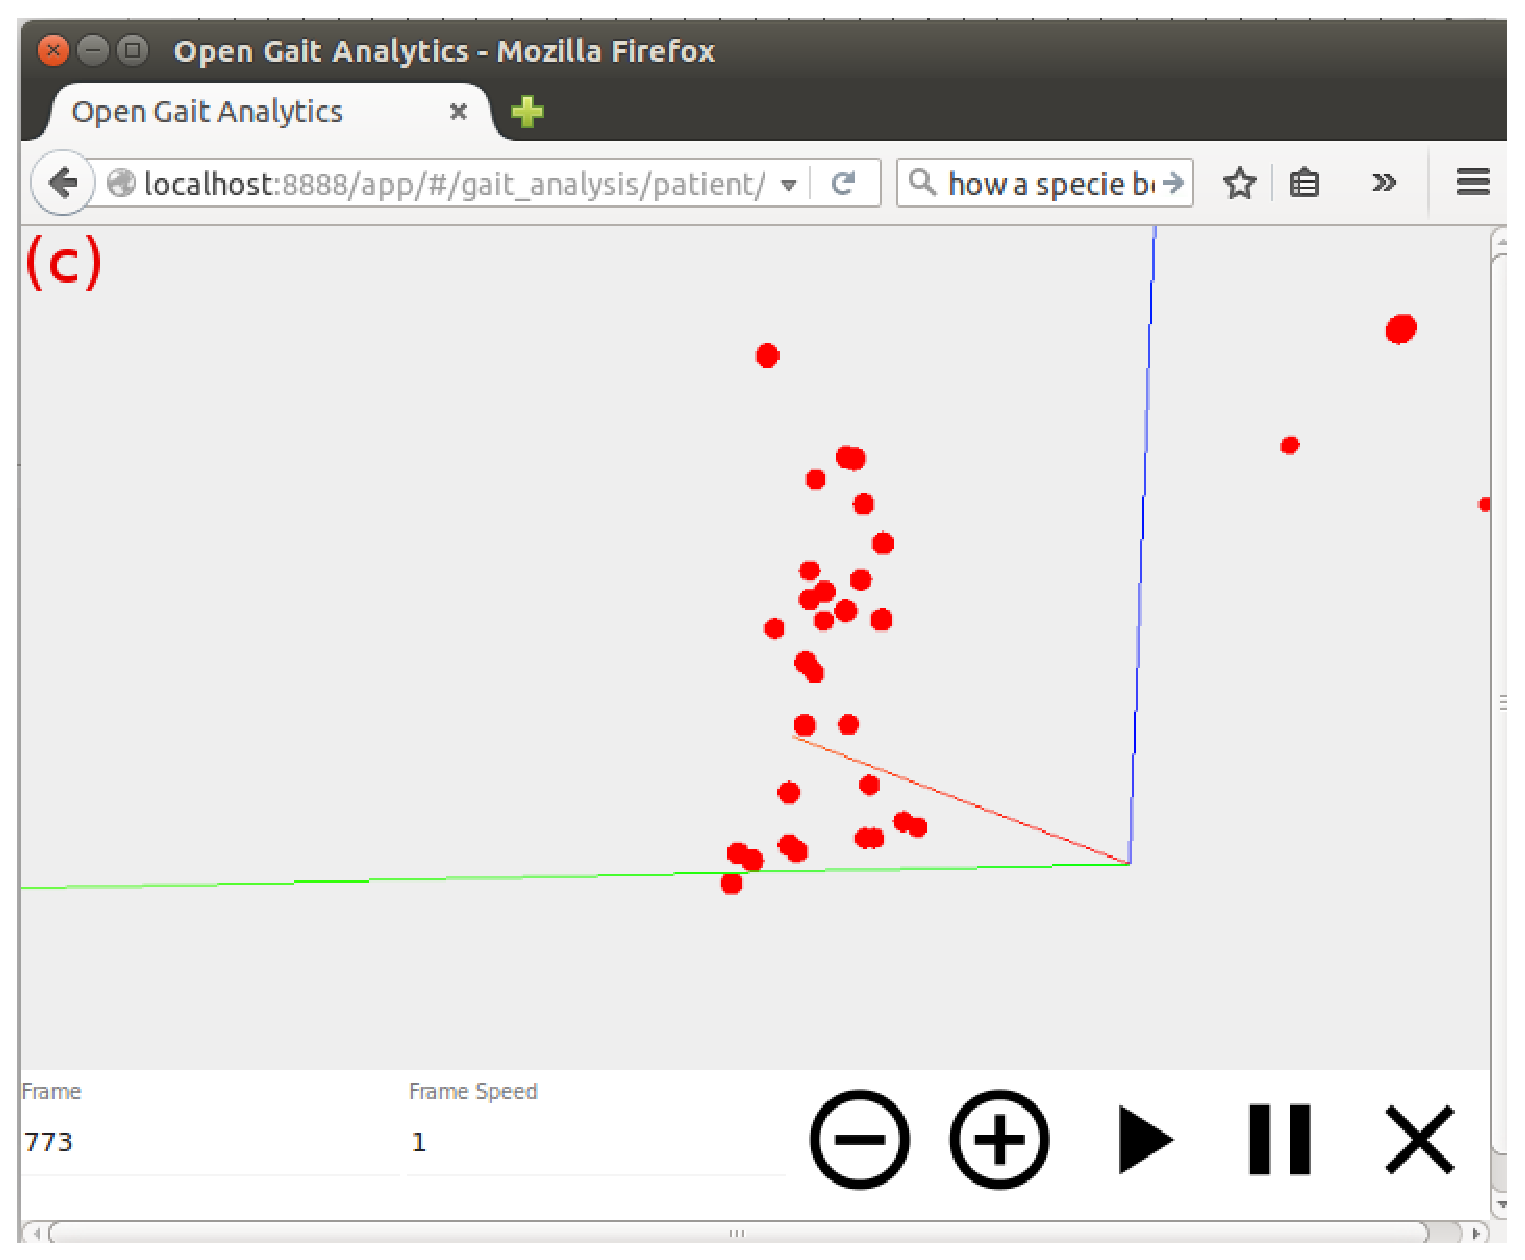
\includegraphics[width=\textwidth]{./animation3.eps}
  \end{minipage}
  \caption{Markers 3D animation. 
	  (a) Left inferior limb initial contact;
	  (b) Left inferior limb terminal instance;
	  (c) Left inferior limb terminal swing.
  }
  \label{animation}
\end{figure*}
\begin{figure}[!t]
	\centering
	{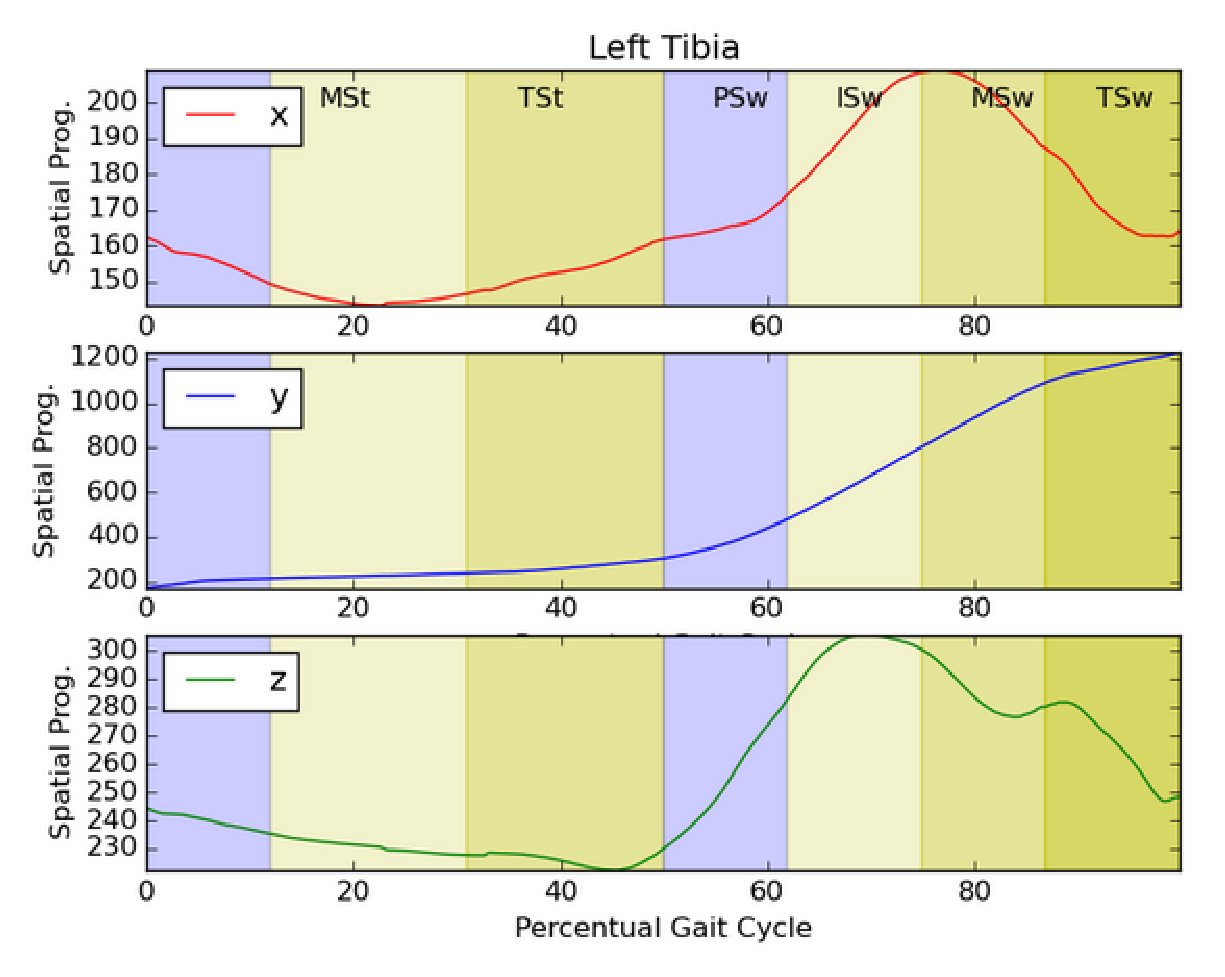
\includegraphics[width=0.48\textwidth]{./spatial_progression.eps}}
	\caption{Left tibial spatial progression.}
	\label{spatial_progression}
\end{figure}


\begin{figure}[!t]
	\centering
	{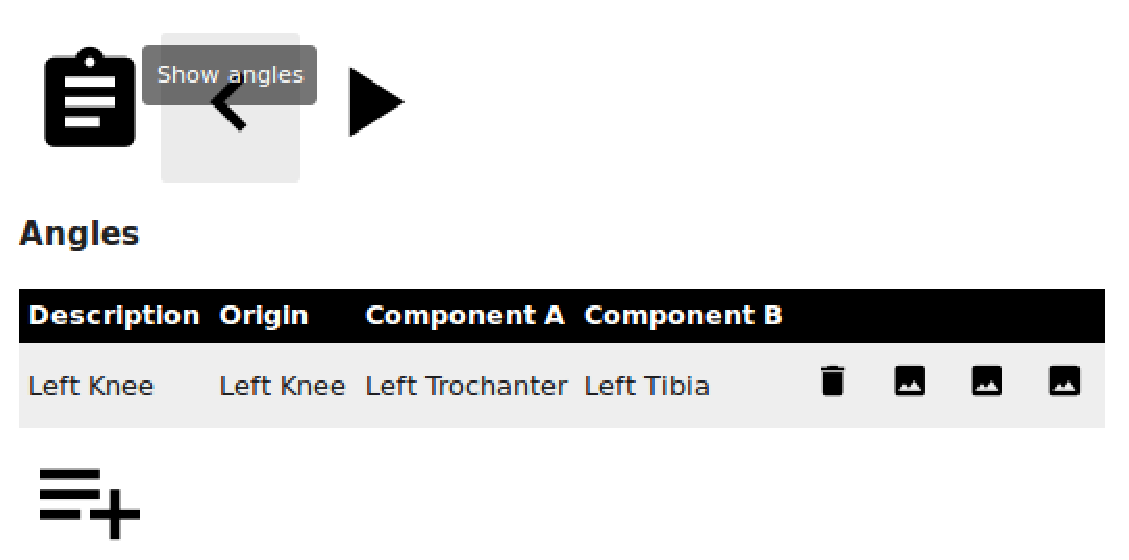
\includegraphics[width=0.46\textwidth]{./angles_tool.eps}}
	\caption{Angle registering tool.}
	\label{angles_tool}
\end{figure}
\begin{figure}[!t]
	\centering
	{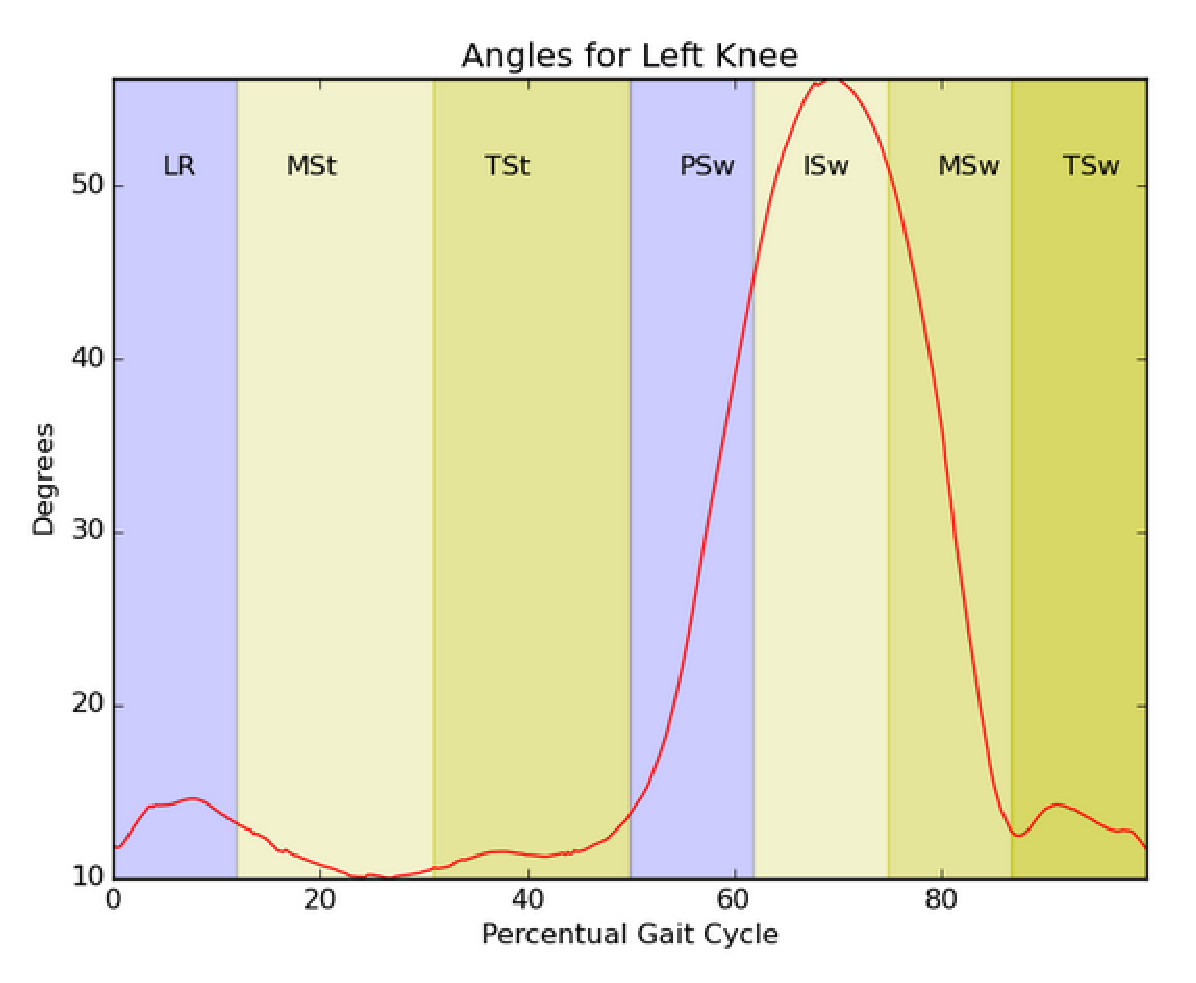
\includegraphics[width=0.49\textwidth]{./angles.eps}}
	\caption{Angles.}
	\label{angles}
\end{figure}
\begin{figure}[!t]
	\centering
	{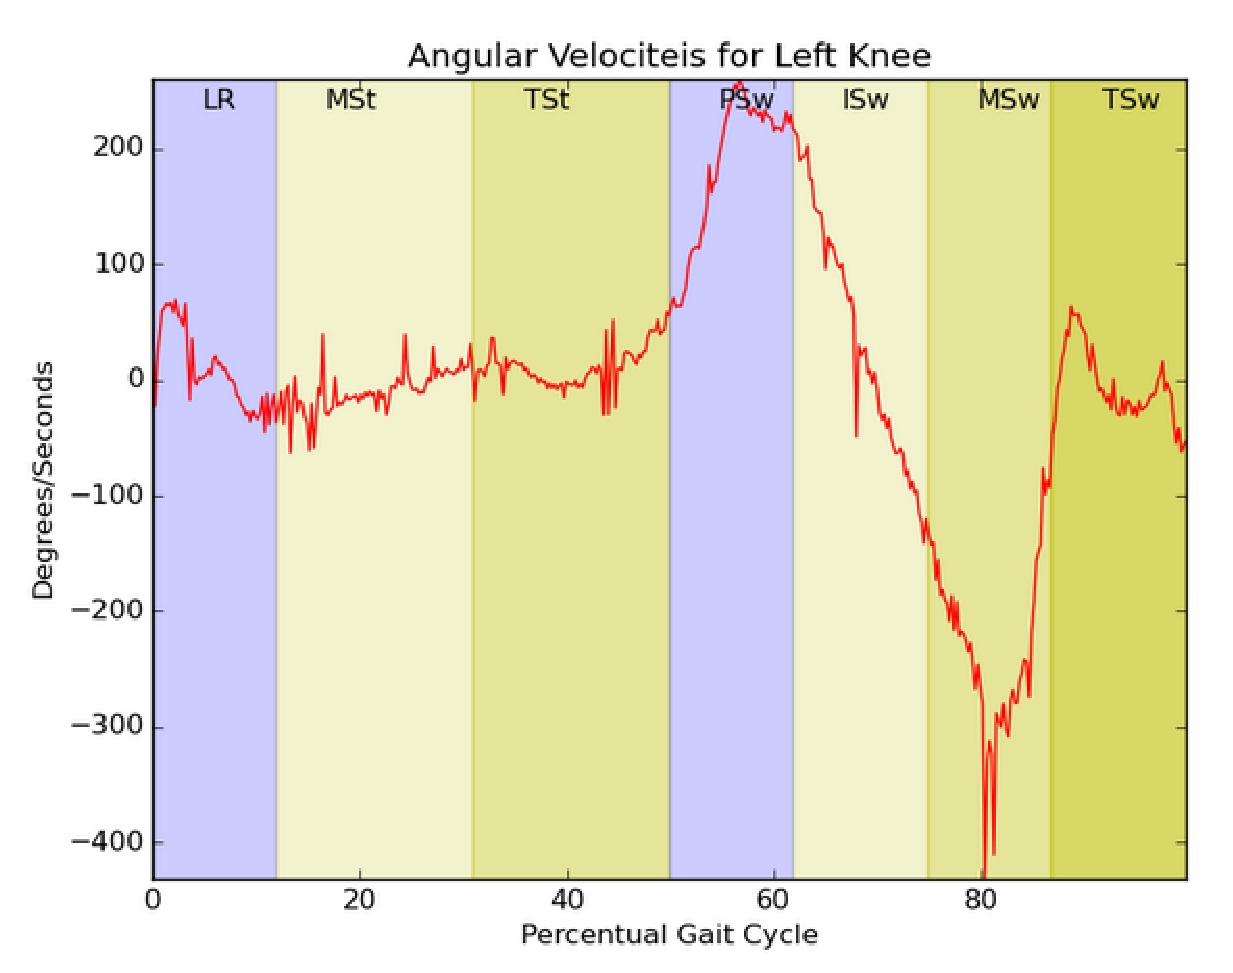
\includegraphics[width=0.49\textwidth]{./av.eps}}
	\caption{Angular velocities.}
	\label{av}
\end{figure}
\begin{figure}[!t]
	\centering
	{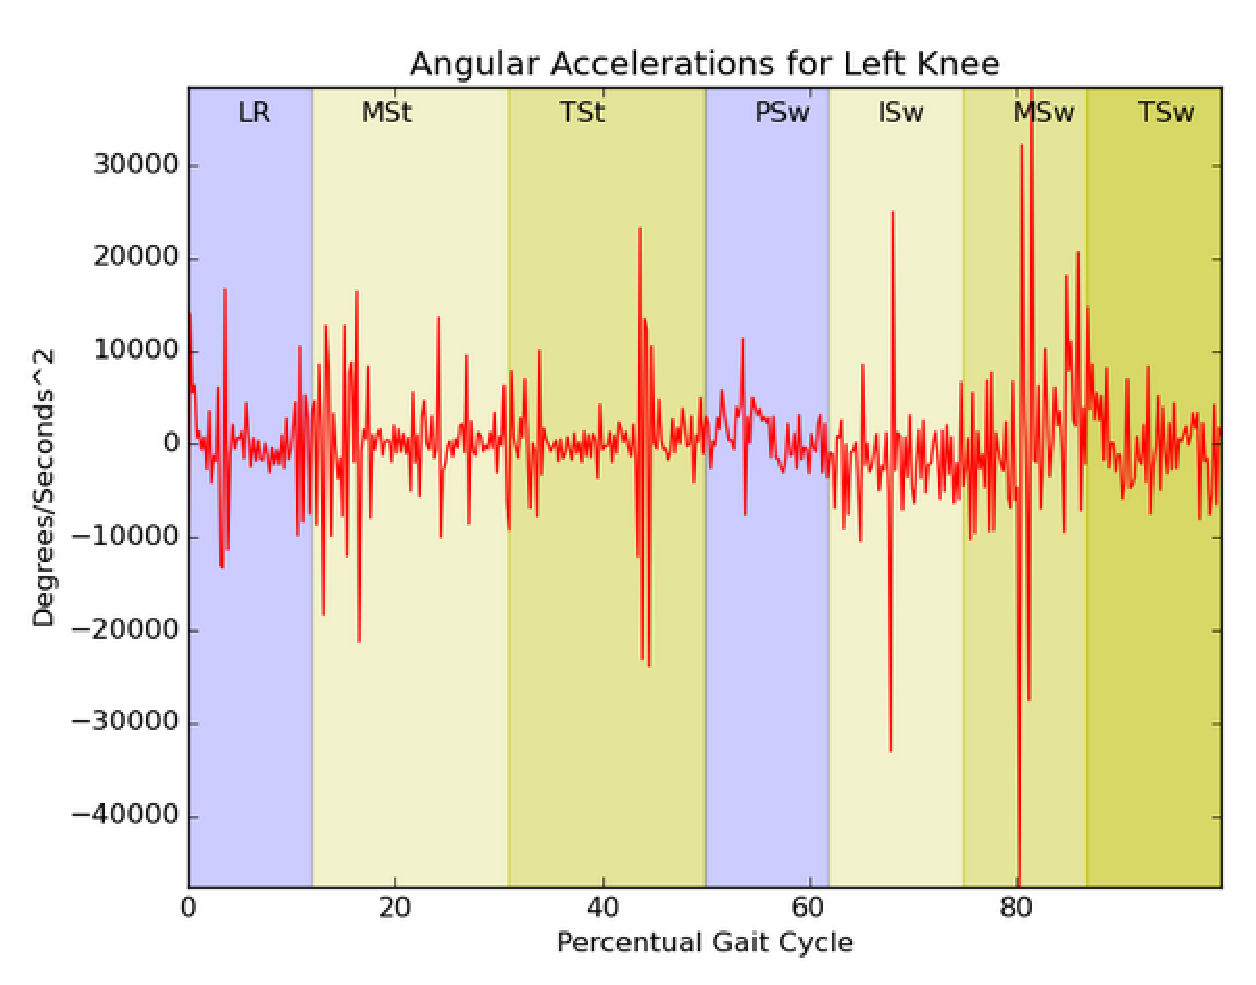
\includegraphics[width=0.49\textwidth]{./aa.eps}}
	\caption{Angular accelerations.}
	\label{aa}
\end{figure}
\begin{figure}[!t]
	\centering
	{\includegraphics[width=0.46\textwidth]{./iphone.eps}}
	\caption{Application running at a mobile phone.}
	\label{iphone}
\end{figure}


% An example of a floating figure using the graphicx package.
% Note that \label must occur AFTER (or within) \caption.
% For figures, \caption should occur after the \includegraphics.
% Note that IEEEtran v1.7 and later has special internal code that
% is designed to preserve the operation of \label within \caption
% even when the captionsoff option is in effect. However, because
% of issues like this, it may be the safest practice to put all your % \label just after \caption rather than within \caption{}.
%
% Reminder: the "draftcls" or "draftclsnofoot", not "draft", class
% option should be used if it is desired that the figures are to be
% displayed while in draft mode.
%
%\begin{figure}[!t]
%\centering
%\includegraphics[width=2.5in]{myfigure}
% where an .eps filename suffix will be assumed under latex, 
% and a .pdf suffix will be assumed for pdflatex; or what has been declared
% via \DeclareGraphicsExtensions.
%\caption{Simulation results for the network.}
%\label{fig_sim}
%\end{figure}

% Note that IEEE typically puts floats only at the top, even when this
% results in a large percentage of a column being occupied by floats.


% An example of a double column floating figure using two subfigures.
% (The subfig.sty package must be loaded for this to work.)
% The subfigure \label commands are set within each subfloat command,
% and the \label for the overall figure must come after \caption.
% \hfil is used as a separator to get equal spacing.
% Watch out that the combined width of all the subfigures on a 
% line do not exceed the text width or a line break will occur.
%
%\begin{figure*}[!t]
%\centering
%\subfloat[Case I]{\includegraphics[width=2.5in]{box}%
%\label{fig_first_case}}
%\hfil
%\subfloat[Case II]{\includegraphics[width=2.5in]{box}%
%\label{fig_second_case}}
%\caption{Simulation results for the network.}
%\label{fig_sim}
%\end{figure*}
%
% Note that often IEEE papers with subfigures do not employ subfigure
% captions (using the optional argument to \subfloat[]), but instead will
% reference/describe all of them (a), (b), etc., within the main caption.
% Be aware that for subfig.sty to generate the (a), (b), etc., subfigure
% labels, the optional argument to \subfloat must be present. If a
% subcaption is not desired, just leave its contents blank,
% e.g., \subfloat[].


% An example of a floating table. Note that, for IEEE style tables, the
% \caption command should come BEFORE the table and, given that table
% captions serve much like titles, are usually capitalized except for words
% such as a, an, and, as, at, but, by, for, in, nor, of, on, or, the, to
% and up, which are usually not capitalized unless they are the first or
% last word of the caption. Table text will default to \footnotesize as
% IEEE normally uses this smaller font for tables.
% The \label must come after \caption as always.
%
%\begin{table}[!t]
%% increase table row spacing, adjust to taste
%\renewcommand{\arraystretch}{1.3}
% if using array.sty, it might be a good idea to tweak the value of
% \extrarowheight as needed to properly center the text within the cells
%\caption{An Example of a Table}
%\label{table_example}
%\centering
%% Some packages, such as MDW tools, offer better commands for making tables
%% than the plain LaTeX2e tabular which is used here.
%\begin{tabular}{|c||c|}
%\hline
%One & Two\\
%\hline
%Three & Four\\
%\hline
%\end{tabular}
%\end{table}


% Note that the IEEE does not put floats in the very first column
% - or typically anywhere on the first page for that matter. Also,
% in-text middle ("here") positioning is typically not used, but it
% is allowed and encouraged for Computer Society conferences (but
% not Computer Society journals). Most IEEE journals/conferences use
% top floats exclusively. 
% Note that, LaTeX2e, unlike IEEE journals/conferences, places
% footnotes above bottom floats. This can be corrected via the
% \fnbelowfloat command of the stfloats package.







% if have a single appendix:
%\appendix[Proof of the Zonklar Equations]
% or
%\appendix  % for no appendix heading
% do not use \section anymore after \appendix, only \section*
% is possibly needed

% use appendices with more than one appendix
% then use \section to start each appendix
% you must declare a \section before using any
% \subsection or using \label (\appendices by itself
% starts a section numbered zero.)
%


%\appendices
%\section{Proof of the First Zonklar Equation}
%Appendix one text goes here.

% you can choose not to have a title for an appendix
% if you want by leaving the argument blank
%\section{}
%Appendix two text goes here.



% Can use something like this to put references on a page
% by themselves when using endfloat and the captionsoff option.
\ifCLASSOPTIONcaptionsoff
  \newpage
\fi



% trigger a \newpage just before the given reference
% number - used to balance the columns on the last page
% adjust value as needed - may need to be readjusted if
% the document is modified later
%\IEEEtriggeratref{8}
% The "triggered" command can be changed if desired:
%\IEEEtriggercmd{\enlargethispage{-5in}}

% references section

% can use a bibliography generated by BibTeX as a .bbl file
% BibTeX documentation can be easily obtained at:
% http://www.ctan.org/tex-archive/biblio/bibtex/contrib/doc/
% The IEEEtran BibTeX style support page is at:
% http://www.michaelshell.org/tex/ieeetran/bibtex/
\bibliographystyle{IEEEtran}
% argument is your BibTeX string definitions and bibliography database(s)
\bibliography{IEEEabrv,./IEEE.bib}
%
% <OR> manually copy in the resultant .bbl file
% set second argument of \begin to the number of references
% (used to reserve space for the reference number labels box)
%\begin{thebibliography}{1}

%\bibitem{IEEEhowto:kopka}
%H.~Kopka and P.~W. Daly, \emph{A Guide to \LaTeX}, 3rd~ed.\hskip 1em plus
%  0.5em minus 0.4em\relax Harlow, England: Addison-Wesley, 1999.

%\end{thebibliography}

% biography section
% 
% If you have an EPS/PDF photo (graphicx package needed) extra braces are
% needed around the contents of the optional argument to biography to prevent
% the LaTeX parser from getting confused when it sees the complicated
% \includegraphics command within an optional argument. (You could create
% your own custom macro containing the \includegraphics command to make things
% simpler here.)
%\begin{IEEEbiography}[{\includegraphics[width=1in,height=1.25in,clip,keepaspectratio]{mshell}}]{Michael Shell}
% or if you just want to reserve a space for a photo:

\begin{IEEEbiography}[{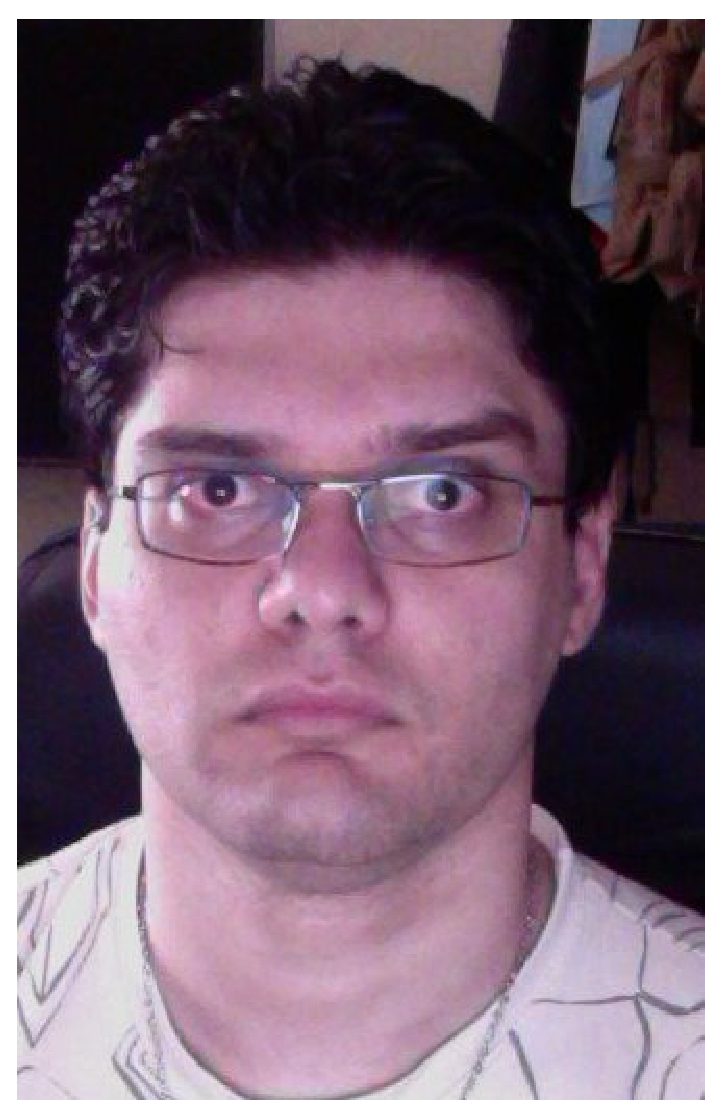
\includegraphics[width=1in,height=1.25in,clip,keepaspectratio]{roberto}}]{Roberto Aguiar Lima}
	is graduated in computer science from Brasilia Catholic University (2000).
	He attends the University of Brasilia Biomedical Engineering M.Sc. Program.
	He has more than twenty years as software developer.

	He is involved in gait analysis research and has interest in machine learning and software engineering.
\end{IEEEbiography}

\begin{IEEEbiography}[{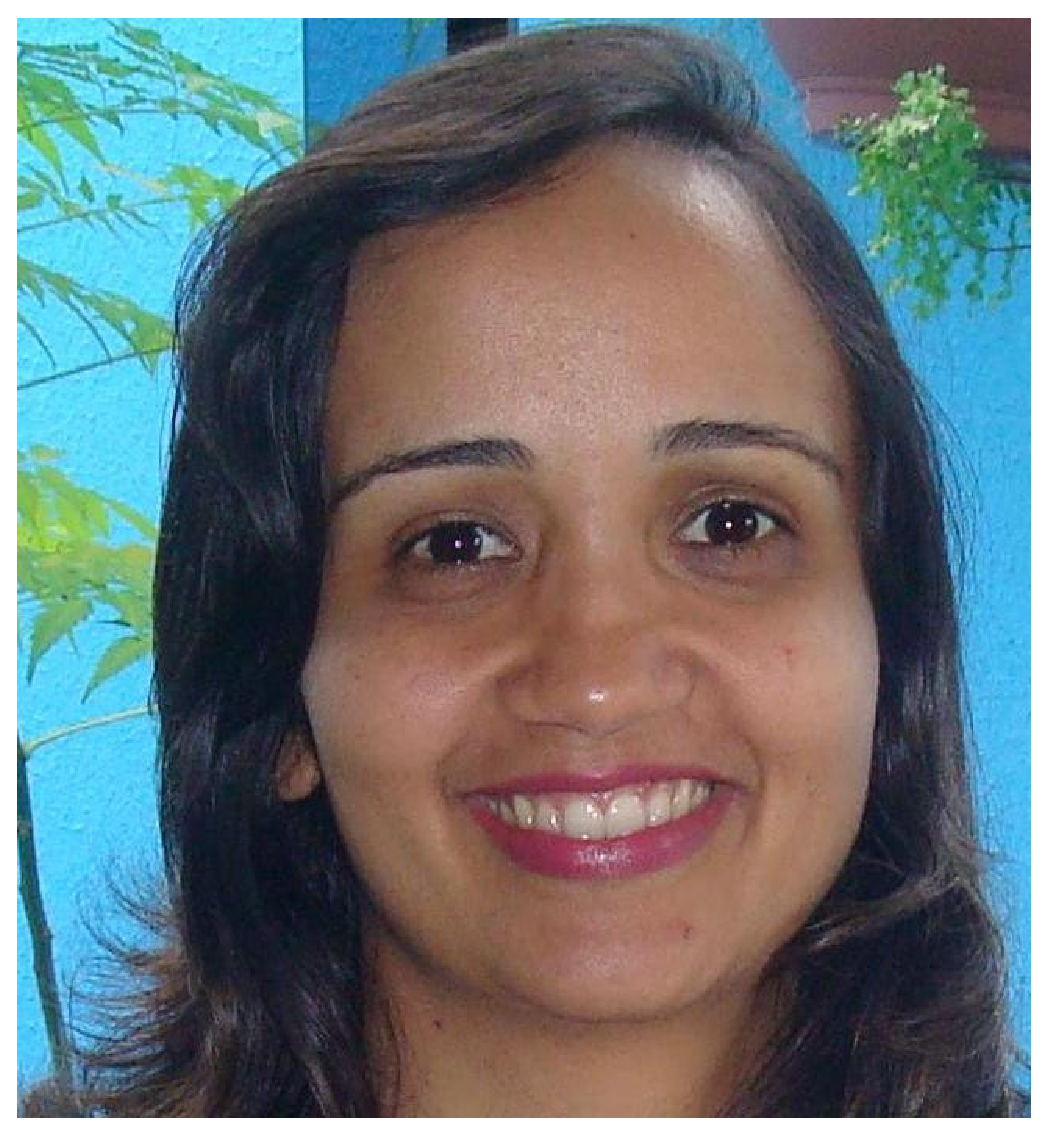
\includegraphics[width=1in,height=1.25in,clip,keepaspectratio]{vera}}]{Vera Regina Fernandes Da Silva Maraes}
	is graduated in physiotherapy by Sao Carlos Federal University (1995). She has a M.Sc. degree in 
	cellular and structural biology by Campinas State University, and a Ph.D. degree in physiotherapy
	from Sao Carlos Federal University. 
	Actually she is  adjunct professor III at: University of Brasilia at Ceilandia; 
	University of Brasilia Biomedical Engineering M.Sc. Program;
	and University of Brasilia Health Pro-Education.

	She has experience in physiotherapy, acting mainly in: health teaching, amputee prosthesis adaptation,
	human functionality, exercise physiology, cardiac rehabilitation and cardiac frequency variability.
\end{IEEEbiography}

\begin{IEEEbiography}[{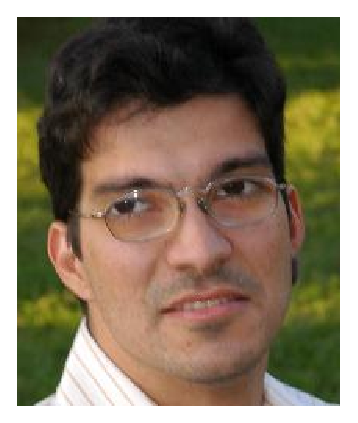
\includegraphics[width=1in,height=1.25in,clip,keepaspectratio]{jairo}}]{Jairo Simao Santana Melo}
Degree in Computer Science from the Catholic University of Brasilia - UCB (2003). Postgraduate in Object Oriented Systems at UCB (2006). Master of Knowledge Management and Technology at UCB (2007), Doctor of Electrical Engineering - Automation (PGEA) at University of Brasilia, UNB (2012). He is currently architect, developer and researcher in the project of Computer Science National Laboratory (LNCC). His scientific works concern: in the navigation area, interaction and visualization of anatomical structures in three-dimensional environment, distributed processing and robotic interfaces (Phantom and Force Dimension) simulating small surgical procedures.
\end{IEEEbiography}

\begin{IEEEbiography}[{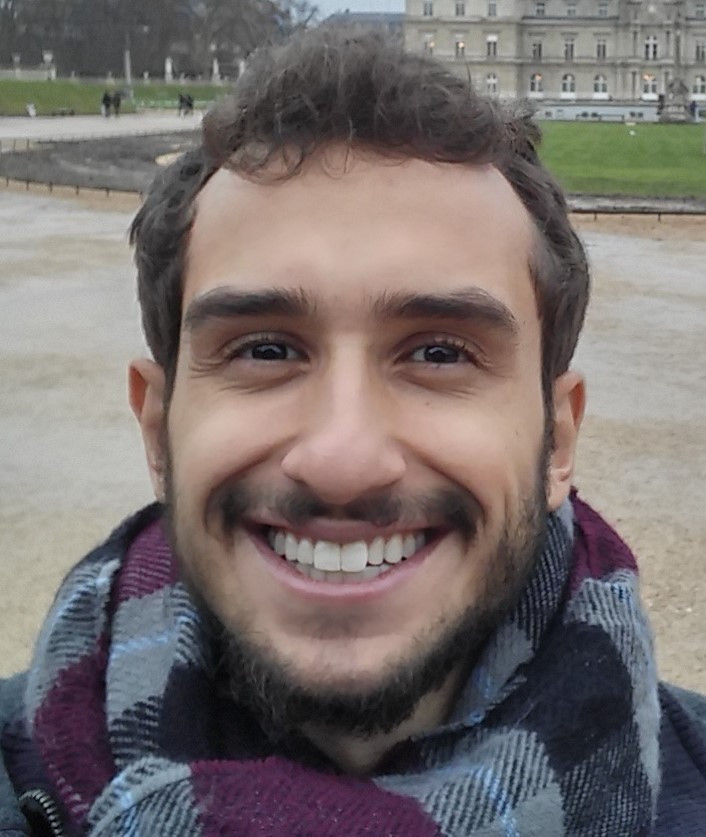
\includegraphics[width=1in,height=1.25in,clip,keepaspectratio]{vladimir}}]{Vladimir Franca Nogueira}
	Graduating in electronic engineer, University of Brasilia (UnB) at Gama (FGA), Brazil. 
	Diploma of business, Imagine Education Australia IEA (2013) Australia. 
	He is currently researcher student in the project of Computer Science National Laboratory (LNCC). 
	His scientific works concern: electronic instrumentation, virtual reality, informatics in health, 
	fuzzy logic, finite element method (FEM), process of deformation on the human breast and robotic 
	interfaces simulating small surgical procedures.
\end{IEEEbiography}


\begin{IEEEbiography}[{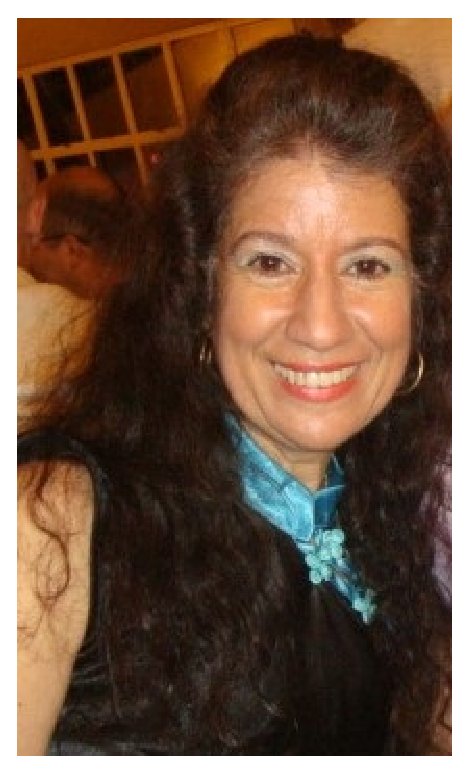
\includegraphics[width=1in,height=1.25in,clip,keepaspectratio]{lourdes}}]{Lourdes Mattos Brasil}.Electrical Engineer, Federal University of
Santa Catarina (1984), Master of Science in Electrical
Engineering/Biomedical Engineering, Federal University of Santa
Catarina (1994), Sandwich Doctorate in Mathematical Applied from
Facultes Universitaires Notre Dame de La Paix (FUNDP), Belgium
(1997–1998) and D.Sc. in Electrical Engineering/Biomedical Engineering
(1999). She is currently professor/researcher/head of the Lato Sensu
in Clinical Engineering Course, besides being professor of the Course
of Electronic Engineering, at the University of Brasilia at Gama,
Brazil. Her scientific works concern: artificial intelligence, data
mining, machine learning, knowledge acquisition, knowledge based
systems, hybrid expert systems, virtual reality, intelligent tutoring
systems, informatics in health, e–learning and nanotechnology.
\end{IEEEbiography}

% insert where needed to balance the two columns on the last page with
% biographies
%\newpage

% a \vfill before or after them. The appropriate
% use of \vfill depends on what kind of text is
% on the last page and whether or not the columns
% are being equalized.

%\vfill

% Can be used to pull up biographies so that the bottom of the last one
% is flush with the other column.
%\enlargethispage{-5in}



% that's all folks
\end{document}
